\documentclass[a4paper,
fontsize=11pt,
%headings=small,
oneside,
numbers=noperiodatend,
parskip=half-,
bibliography=totoc,
final
]{scrartcl}

\usepackage[babel]{csquotes}
\usepackage{synttree}
\usepackage{graphicx}
\setkeys{Gin}{width=.4\textwidth} %default pics size

\graphicspath{{./plots/}}
\usepackage[ngerman]{babel}
\usepackage[T1]{fontenc}
%\usepackage{amsmath}
\usepackage[utf8x]{inputenc}
\usepackage [hyphens]{url}
\usepackage{booktabs} 
\usepackage[left=2.4cm,right=2.4cm,top=2.3cm,bottom=2cm,includeheadfoot]{geometry}
\usepackage[labelformat=empty]{caption} % option 'labelformat=empty]' to surpress adding "Abbildung 1:" or "Figure 1" before each caption / use parameter '\captionsetup{labelformat=empty}' instead to change this for just one caption
\usepackage{eurosym}
\usepackage{multirow}
\usepackage[ngerman]{varioref}
\setcapindent{1em}
\renewcommand{\labelitemi}{--}
\usepackage{paralist}
\usepackage{pdfpages}
\usepackage{lscape}
\usepackage{float}
\usepackage{acronym}
\usepackage{eurosym}
\usepackage{longtable,lscape}
\usepackage{mathpazo}
\usepackage[normalem]{ulem} %emphasize weiterhin kursiv
\usepackage[flushmargin,ragged]{footmisc} % left align footnote
\usepackage{ccicons} 
\setcapindent{0pt} % no indentation in captions
\usepackage{xurl} % Breaks URLs

%%%% fancy LIBREAS URL color 
\usepackage{xcolor}
\definecolor{libreas}{RGB}{112,0,0}

\usepackage{listings}

\urlstyle{same}  % don't use monospace font for urls

\usepackage[fleqn]{amsmath}

%adjust fontsize for part

\usepackage{sectsty}
\partfont{\large}

%Das BibTeX-Zeichen mit \BibTeX setzen:
\def\symbol#1{\char #1\relax}
\def\bsl{{\tt\symbol{'134}}}
\def\BibTeX{{\rm B\kern-.05em{\sc i\kern-.025em b}\kern-.08em
    T\kern-.1667em\lower.7ex\hbox{E}\kern-.125emX}}

\usepackage{fancyhdr}
\fancyhf{}
\pagestyle{fancyplain}
\fancyhead[R]{\thepage}

% make sure bookmarks are created eventough sections are not numbered!
% uncommend if sections are numbered (bookmarks created by default)
\makeatletter
\renewcommand\@seccntformat[1]{}
\makeatother

% typo setup
\clubpenalty = 10000
\widowpenalty = 10000
\displaywidowpenalty = 10000

\usepackage{hyperxmp}
\usepackage[colorlinks, linkcolor=black,citecolor=black, urlcolor=libreas,
breaklinks= true,bookmarks=true,bookmarksopen=true]{hyperref}
\usepackage{breakurl}

%meta
%meta

\fancyhead[L]{K. Schuldt\\ %author
LIBREAS. Library Ideas, 45 (2024). % journal, issue, volume.
\href{https://doi.org/10.18452/...}{\color{black}https://doi.org/10.18452/...}
{}} % doi 
\fancyhead[R]{\thepage} %page number
\fancyfoot[L] {\ccLogo \ccAttribution\ \href{https://creativecommons.org/licenses/by/4.0/}{\color{black}Creative Commons BY 4.0}}  %licence
\fancyfoot[R] {ISSN: 1860-7950}

\title{\LARGE{Musik und Volksbüchereien in Deutschland, 1900–1945}}% title
\author{Karsten Schuldt} % author

\setcounter{page}{1}

\hypersetup{%
      pdftitle={Musik und Volksbüchereien in Deutschland, 1900–1945},
     pdfauthor={Karsten Schuldt},
      pdfcopyright={CC BY 4.0 International},
      pdfsubject={LIBREAS. Library Ideas, 45 (2024).},
      pdfkeywords={Musikbücherei, Musikbibliothek, Bibliotheksgeschichte, Weimarer Republik, Nationalsozialismus, Musikalien},
      pdflicenseurl={https://creativecommons.org/licenses/by/4.0/},
      pdfurl={https://doi.org/10.18452/...},
      pdfdoi={10.18452/...},
      pdflang={de},
      pdfmetalang={de}
     }



\date{}
\begin{document}

\maketitle
\thispagestyle{fancyplain} 

%abstracts
\begin{abstract}
\noindent
\textbf{Abstract:} Die Frage, ob «Musikalien» wie Noten oder
Musikliteratur Teil der Volksbüchereien, also der Vorgänger der heutigen
Öffentlichen Bibliotheken, sein sollten, wurde schon ganz am Anfang des
(deutschen) Volksbüchereiwesens gestellt. Grundsätzlich wurde dies
schnell bejaht und bald angefangen, eigenständige Musikabteilungen und
Öffentliche Musikbüchereien einzurichten. Von 1900 bis 1945 erschien zu
diesem Themenkomplex in der deutschen bibliothekarischen Fachliteratur
eine überschaubare, aber doch beachtliche Zahl von Texten. Diese werden
hier in chronologischer Reihenfolge vorgestellt. Sichtbar wird dabei,
dass sich Volksbüchereien und deren Musikabteilungen gemeinsam
entwickelten, aber auch, dass diese Entwicklung immer eingelassen war in
der Entwicklung der deutschen Gesellschaft.

\textbf{Abstract:} The question of whether ``musicalia'' such as sheet
music or music literature should be part of the ``Volksbüchereien'',
i.e.~the predecessors of today's public libraries, was raised at the
very beginning of the (German) Volksbücherei movement. In principle,
this was quickly answered in the affirmative. Soon, independent music
departments and public music libraries were set up. From 1900 to 1945, a
manageable but considerable number of texts concerning this topical
field appeared in German library literature. These are presented here in
chronological order. It becomes clear that the Volksbüchereien and their
music departments developed together, but that this development was also
always embedded in the development of German society.
\end{abstract}

%body
\hypertarget{musikalien-und-volksbuxfcchereien-eine-fruxfche-entwicklung}{%
\section{1. Musikalien und Volksbüchereien -- Eine frühe
Entwicklung}\label{musikalien-und-volksbuxfcchereien-eine-fruxfche-entwicklung}}

Die der damaligen «Volksbildungsbewegung» zuzuordnenden Volksbüchereien
und Lesehallen, welche Ende des 19. und Anfang des 20. Jahrhunderts
entstanden, sind (neben den «katholischen Volksbüchereien» (Zalar 2019),
den sozialdemokratischen «Arbeiterbibliotheken» sowie den gewerblichen
«Leihbibliotheken») die hauptsächlichen Einrichtungen, aus denen sich im
Laufe des 20. Jahrhunderts die heutigen Öffentlichen Bibliotheken im
DACH-Raum entwickelten. Die erste Zeitschrift, welche sich explizit den
Einrichtungen der «Volksbüchereibewegung» widmete, waren die
\emph{Blätter für Volksbüchereien und Lesehallen}, die im Januar 1900
das erste Mal erschien.\footnote{Genaugenommen erschien sie zuerst als
  Beilage des \emph{Zentralblatt für Bibliothekswesen}. Das Erscheinen
  zeigt also auch den Beginn einer Trennung der Bibliothekstypen an, die
  heute als Öffentliche respektive Wissenschaftliche Bibliotheken (die
  weiterhin im \emph{Zentralblatt} publizierten) bezeichnet werden.}
Über die gesamte Zeit ihres Erscheinens, bis 1919, begann jede Ausgabe
auf der ersten Seite, direkt unter dem Titelkopf mit Namen,
Ausgabennummer und Impressum, ohne weitere Einleitung mit dem ersten
Artikel. In der ersten Nummer war dies ein Text, mit dem die Zeitschrift
selber vorgestellt wurde. (Der Herausgeber 1900) Aber gleich in der
zweiten Nummer, erschienen im März 1900, stand als Titel dieses ersten
Textes die Frage «Gehören Musikalien in die Bücherhallen?». (Altmann
1900) Das ist kein Zufall.

Das Thema Musik trieb die Volksbüchereibewegung schon sehr kurz nach
ihrer Entstehung um. Nach den gedruckten Büchern, später dann Zeitungen
und Zeitschriften, die als «Hauptmedien» der Volksbüchereien angesehen
wurden, waren «Musikalien» -- also vor allem Notendrucke -- und kurz
danach Schallplatten praktisch die ersten Medienformen, welche eine
besondere Betrachtung durch die Volksbüchereien erhielten. Sollten sie
in die Büchereien aufgenommen werden oder nicht? War die Musik eine
Aufgabe von Volksbüchereien -- und wenn ja, was für eine Aufgabe genau,
mit welchem Ziel? Das Gleiche geschah in der Veranstaltungsarbeit der
Volksbüchereien. Schon früh beschäftigte sich die Volksbüchereibewegung
mit der Frage, welche Veranstaltungen von den Büchereien durchgeführt
werden sollten und welche Veranstaltungen anderer Einrichtungen --
beispielsweise die der zu dieser Zeit neu entstehenden Volkshochschulen
oder in Österreich der «Universitätsausdehnungsbewegung» (Pöggeler 1974)
-- man unterstützen sollte. Dabei ging es wieder zuerst um Bücher und
Literatur. Aber nicht lange danach wurden auch Stimmen laut, die
Konzerte und musikalische Lehrvorträge forderten. (Ackerknecht 1930)
Oder aber solche, die Vorlesestunden mit Liedern von Schallplatten
anreichern wollten. (Ackerknecht 1926) Nachdem ab ungefähr 1910 in den
ersten Volksbüchereien und Lesehallen, für die extra eigene Gebäude
errichtet wurden, Vortragssäle eingerichtet worden waren, kam
folgerichtig schnell die Forderung auf, auch Konzert- und Musikzimmer
einzurichten. (Bayer 1931)

Immer folgte in der Volksbüchereibewegung die Musik recht bald der
Literatur. Es war nie das Hauptthema der Fachliteratur oder der
Büchereien -- immer waren es nur wenige Artikel, wenige
Musikabteilungen, wenige Ressourcen, die für Musikalien aufgebracht
wurden, wenn man sie ins Verhältnis zum gesamten Volksbüchereiwesen
setzt. Und immer wieder wurde dabei die Frage, welche 1900 im ersten
Artikel gestellt wurde, nämlich die nach der Bedeutung von Musik für die
Büchereien, neu gestellt. Und trotzdem kann man auch erkennen, dass dem
Thema grundsätzlich viel Wohlwollen entgegengebracht wurde. Es wurde
früh auf die Tagesordnung gehoben und ihm wurde immer wieder Platz
eingeräumt, in der Presse der Volksbüchereien, auf den Tagungen und auch
in einzelnen Büchereien selber. Musik in der Volksbücherei ist ein
Thema, dass sich zusammen mit der deutschen Volksbüchereibewegung
mitentwickelt hat.

Der vorliegende Text soll dies anhand der Publikationen, die bis 1945 in
der Fachliteratur für Volksbüchereien in Deutschland erschienen sind,
nachzeichnen. (Schön wäre es, dem auch Artikel aus dem restlichen
deutschsprachigen Raum gegenüberstellen zu können, um Unterschiede und
Gemeinsamkeiten herauszuarbeiten. Aber, soweit recherchierbar, sind
solche Artikel nicht erschienen.) 1945 ist ein Datum, das wegen des
Endes des Nationalsozialismus und des Zweiten Weltkrieges im DACH-Raum
oft als Zäsur genommen wird. Es bietet sich aber für das Thema dieses
Artikels auch an, weil die Volksbüchereibewegung als solche nach 1945
langsam endete. Durch den nationalsozialistischen Staat waren die
Büchereien als Einrichtungen explizit den Gemeinden zugeordnet, die
Arbeiterbibliotheken aufgelöst und die katholischen in ihrer Bedeutung
reduziert worden. Auf dieser Situation aufbauend, aber unter ganz
anderen politischen Vorzeichen, wurden in den Besatzungszonen, später
der BRD, der DDR und Österreich nach 1945 neue Formen der Büchereien
entwickelt. Sie wurden über die folgenden Jahrzehnte von den
Volksbüchereien zu den heutigen modernen Öffentlichen Bibliotheken. In
der Schweiz und Liechtenstein entwickelte sich dies ähnlich, aber ohne
politischen Zwang und teilweise zeitversetzt. Mit diesen Entwicklungen
nach 1945 ging, nach den ersten Aufbaujahren, ein massives Wachstum der
bibliothekarischen Publikationen und damit auch von Artikeln zum Thema
Musik und Büchereien einher. Gleichzeitig organisierten sich die
Musikbibliotheken und professionalisierten sich. 1952 wurde (in der BRD)
die heutige deutsche Gruppe der \emph{International Association of Music
Libraries, Archives and Documentation Centres} gegründet, zu der auch
die Öffentlichen Musikbibliotheken gehören. Seit 1980 existiert für
diese Bibliotheken mit dem \emph{Forum Musikbibliothek} auch eine eigene
Zeitschrift. Oder anders gesagt: Nach 1945 war das Öffentliche
Bibliothekswesen ein anderes, das sich auch nicht mehr einfach mit dem
aus der Zeit vor dem Nationalsozialismus vergleichen lässt. Dies gilt
auch für die Öffentlichen Musikbibliotheken. Deshalb werden deren
Entwicklungen nach 1945 in diesem Artikel nicht genauer betrachtet.

Gleichzeitig beschränkt sich dieser Text auf die Artikel, die in der
bibliothekarischen Literatur erschienen sind. In der Literatur, die sich
mit Musik beschäftigt, sind gewiss weitere Texte erschienen, die sich
auf Musikbüchereien bezogen. Deren Sichtung und Kontextualisierung muss
eine offene Aufgabe bleiben. (Zu sagen ist aber, dass solche in den hier
vorgestellten Texten fast nicht referenziert werden. Nur der weiter
unten angeführte Text von Walter Hofmann und Konrad Ameln (Hofmann \&
Ameln 1927) verweist explizit auf solche.)

Aufgebaut ist dieser Artikel nun wie folgt: Nach der gerade gelieferten
Einleitung (1) wird im folgenden Kapitel chronologisch berichtet, was in
Texten über Musik und Büchereien, die bis 1933 erschienen, jeweils
thematisiert wurde. Es sind nicht so viele, dass es sich anbieten würde,
sie weiter zusammenzufassen. Die Chronologie bietet sich aber an, weil
in vielen dieser Artikel tatsächlich auf vorhergehende Texte Bezug
genommen wird, sie also selber als Teil einer Entwicklung verortet
werden. (2) Nach 1933 ändert sich der Kontext dieser Texte, aber auch
die Texte selber: Dem Singen und der Musik, insbesondere der populären
Musik (Volkslieder und Marschlieder) wurde im Nationalsozialismus ein
besonderer Status eingeräumt (Nierenz 2010), der sich auch im Ausbau von
Infrastruktur niederschlug. Diese Infrastruktur umfasste zum Beispiel
Singegruppen in \emph{Hitlerjugend} und \emph{Bund Deutscher Mädel}, der
Aufwertung das Fachs «Musik» an den grundständigen Schulen (wobei hier,
trotz aller anderen Verlautbarungen, an Entwicklungen aus der Weimarer
Republik angeschlossen wurde), aber neue Musikabteilungen in
Volksbüchereien. Gleichzeitig blieb es nicht bei dieser Infrastruktur,
sondern im Alltag des Nationalsozialismus etablierte sich das Singen als
Tätigkeit vieler Menschen und gewann eine neue Bedeutung: Viele Menschen
sangen tatsächlich\footnote{Die Aussage hier bezieht sich auf «die
  normale Bevölkerung». Aber selbstverständlich gehört zum
  Nationalsozialismus auch, dass beispielsweise Menschen, die in die
  Konzentrationslager verbracht wurden, dort teilweise zum Singen
  gezwungen wurden. Auch der Horror des nationalsozialistischen Terrors
  wurde mit Musik und Gesang verbunden, beziehungsweise wurde gerade
  Musik und erzwungenes Singen teilweise als Folterwerkzeug oder Mittel
  der Demütigung eingesetzt. (Klause 2021, Fackler 2000) Gleichzeitig
  waren es nicht nur die Nationalsozialist*innen, welche Musik nutzten.
  Auch ihre Opfer machten selbstbestimmte Musik, sowohl mit
  politisch-kämpferischer Absicht als auch als Möglichkeit, die eigene
  Identität zu bewahren, Haft und Lager zu überstehen oder zur
  Unterhaltung. (Klause 2021, Gilbert 2005, Fackler 2000) Stoverock
  (2013) erwähnt explizit, dass sich das Liedgut von Täter*innen und
  Opfern des Nationalsozialismus in grossen Teilen überschnitt, schon
  weil Lieder oft auf der Basis vorhandener Melodien getextet wurden.
  Sichtbar wird all dies in den Texten zu Musikbüchereien aber nicht.}
(Niessen 1999) und einige davon hatten offenbar auch ein Interesse an
den Angeboten von Volksbüchereien. Dies zeigte sich auch in den
bibliothekarischen Texten. Nach einigen programmatischen Texten finden
sich in der Literatur deshalb immer mehr Beiträge und kurze Notizen, die
von der Gründung von Musikabteilungen berichten, insbesondere während
des Zweiten Weltkrieges. Deshalb wird bei der Darstellung der Texte aus
dem Nationalsozialismus der chronologischen Darstellung gefolgt, aber
die zuletzt erschienenen werden zusammengefasst. (3) Im anschliessenden
Kapitel (4) wird ein kurzer Ausblick auf die weitere Entwicklung der
Musikbüchereien geworfen. Im Fazit (5) werden noch einmal die grossen
Entwicklungslinien nachgezogen und gefragt, ob sie heute noch erkennbar
sind.

\begin{figure}
\centering
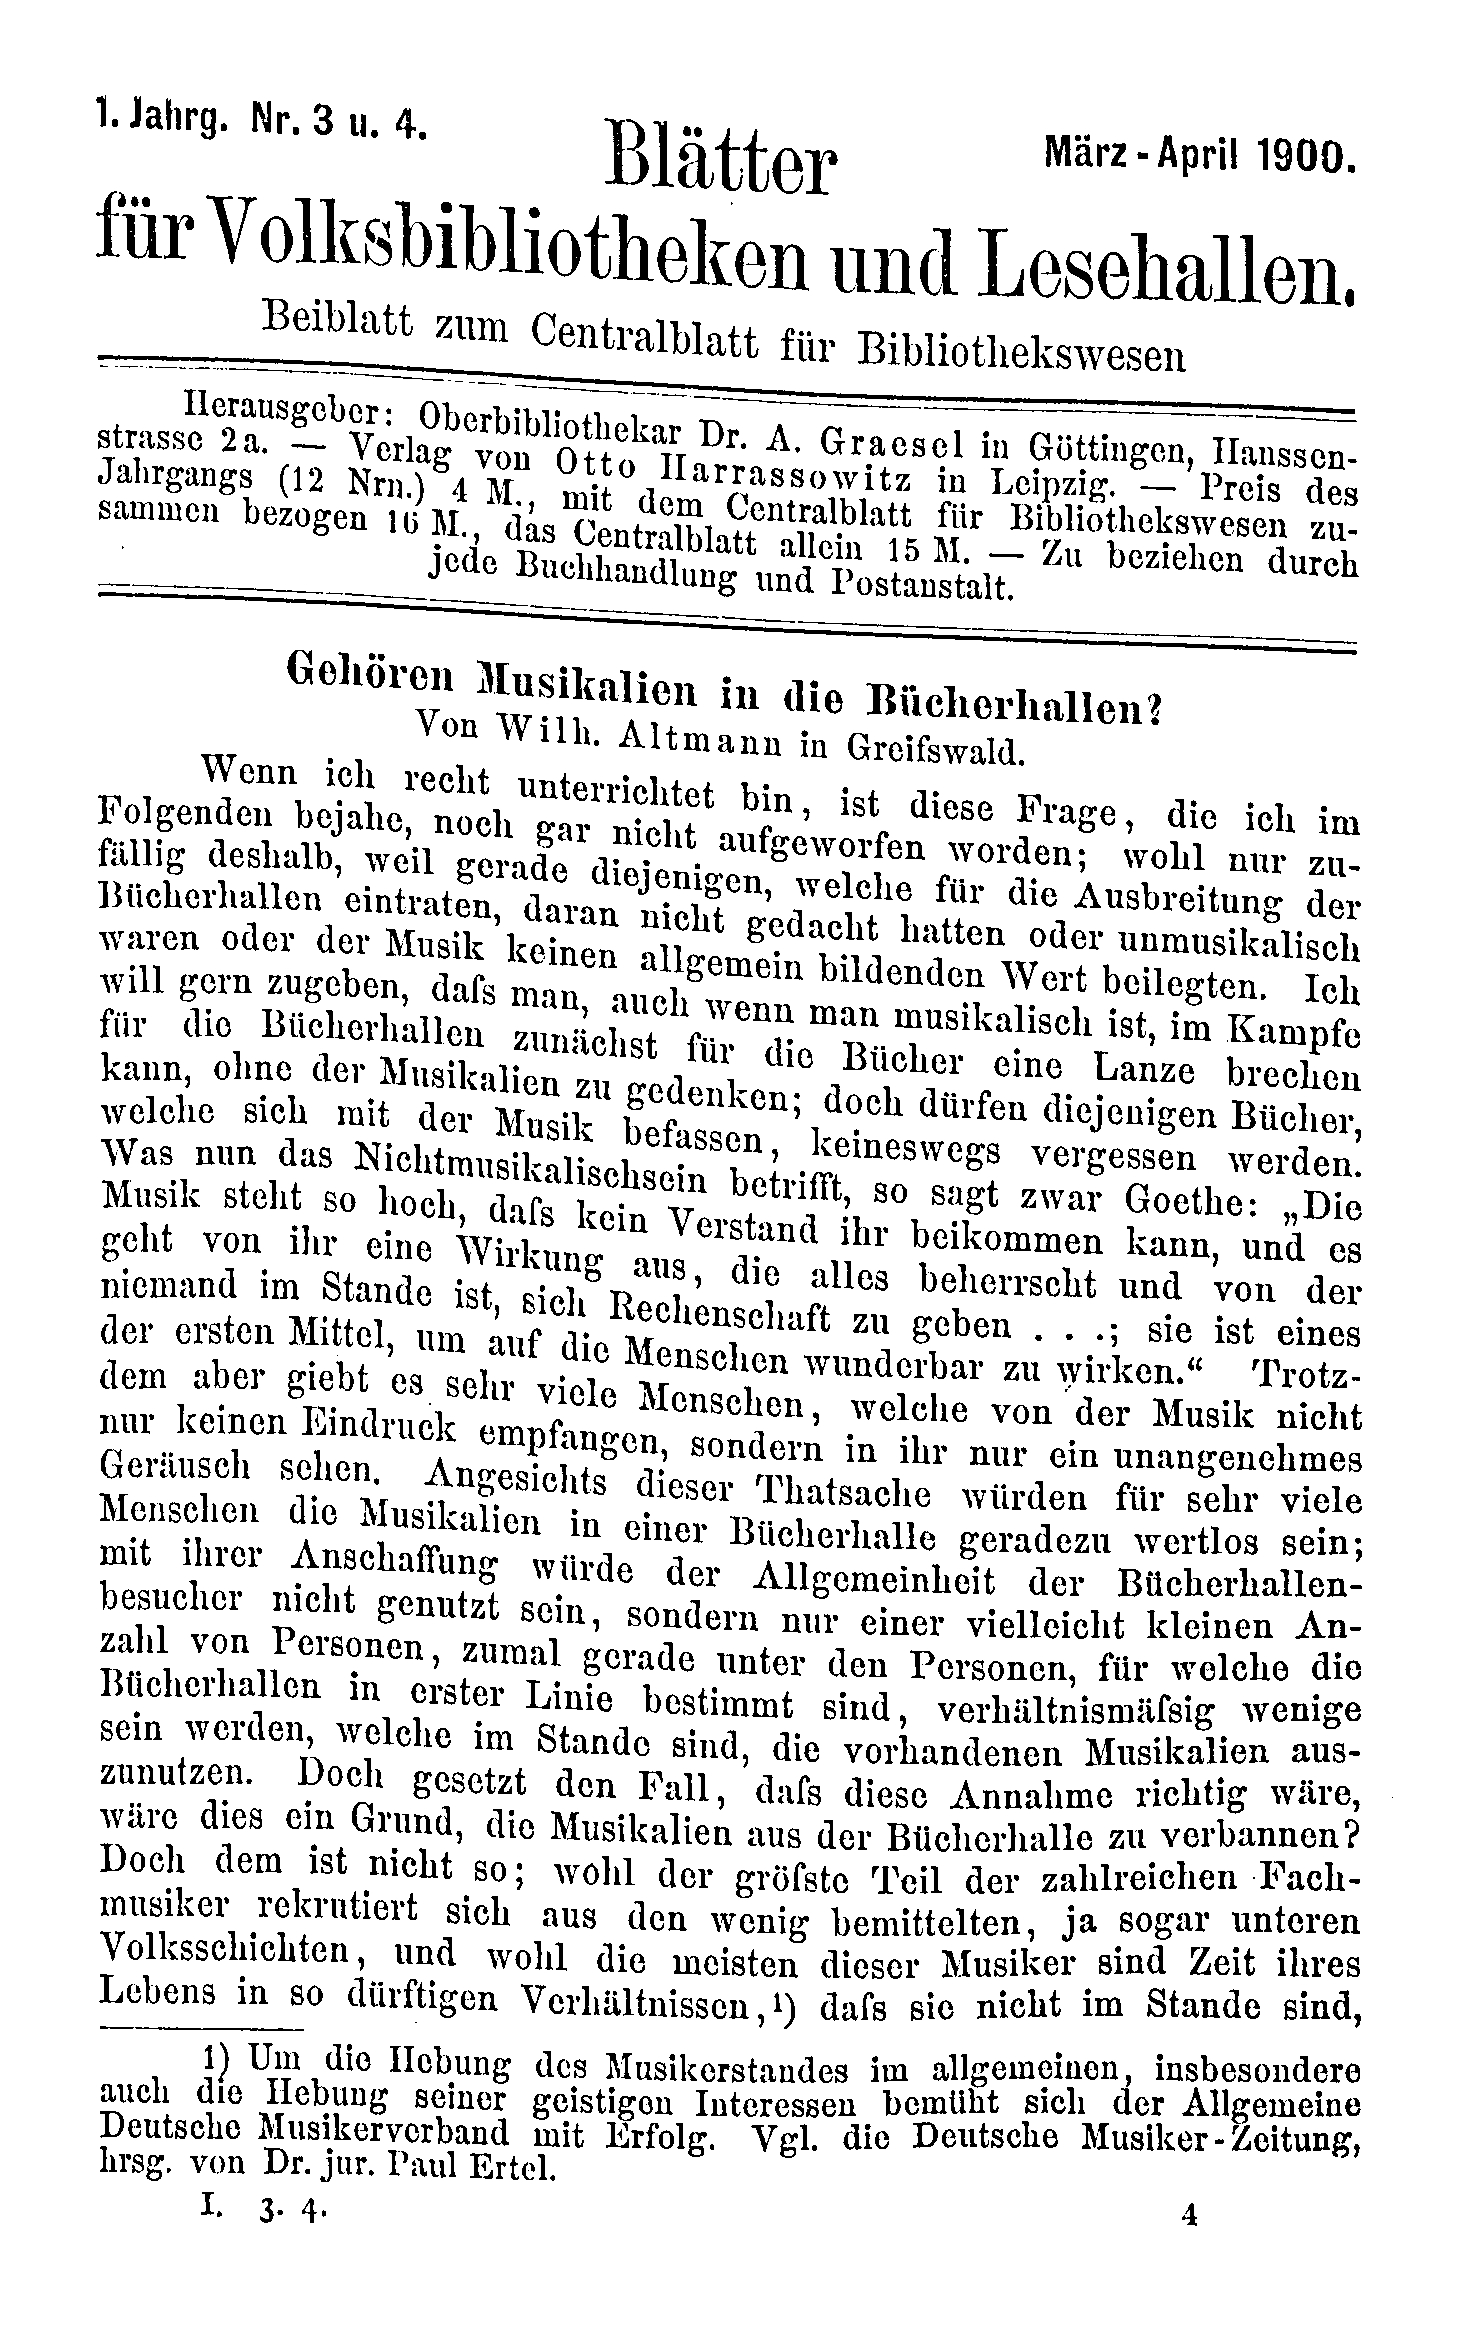
\includegraphics{files/Altmann_1900.jpg}
\caption{Titelseite von Altmann (1900)}
\end{figure}

\hypertarget{kaiserreich-und-weimarer-republik}{%
\section{2. Kaiserreich und Weimarer
Republik}\label{kaiserreich-und-weimarer-republik}}

\hypertarget{gehuxf6ren-musikalien-in-die-buxfccherhallen-1900}{%
\subsection{2.1 Gehören Musikalien in die Bücherhallen?
(1900)}\label{gehuxf6ren-musikalien-in-die-buxfccherhallen-1900}}

Wie erwähnt erschien der erste Text, welcher sich im DACH-Raum mit der
Frage beschäftigte, wie das Verhältnis von Musik und Büchereien sein
sollte, im Jahr 1900. Der Autor, Wilhelm Altmann, beginnt im Titel zwar
mit der Frage, ob Musikalien -- das sind bei ihm Notendrucke und
Literatur zum Lernen des Musizierens -- in den Volksbüchereien vorhanden
sein sollten. Aber es wird in dem Text schnell klar, dass diese Frage
für ihn von Anfang an mit einem «Ja» zu beantworten ist. Anstatt sie
abzuwägen und zu diskutieren, versammelt er hier nur Argumente dafür.

Dass er dabei für die Einrichtungen, über die er schreibt, die
Bezeichnung «Bücherhallen» nutzt, ist ein Hinweis auf die gewisse
Offenheit der Entwicklung, die 1900 noch das gesamte Volksbüchereiwesen
auszeichnete. Man könnte das Wort als Zusammenführung der im Namen der
Zeitschrift \emph{Blätter für Volksbüchereien und Lesehallen} genannten
Einrichtungen lesen. Das waren damals tatsächlich zwei unterschiedliche,
wenn auch eng verwandte Einrichtungen: In Büchereien wurden Bücher
verliehen. Immer mit einem erzieherischen Anspruch und immer als
Thekenbibliotheken -- also mit einer Trennung zwischen Leser*innen und
Bestand durch eine Theke, hinter der Bibliothekar*innen standen, welche
die Ausleihe mit Beratung, Erziehung oder (je nachdem, wie man es
bewertet) Überwachung der Leser*innen verbanden. Gelesen wurde in diesen
Büchereien um 1900 aber nicht. In Lesehallen hingegen wurden Bücher als
Präsenzbestand gehalten, also explizit nicht verliehen. Leser*innen
kamen in die Lesehallen, um diese Bücher zu lesen. Im Laufe der nächsten
Jahrzehnte ging dann offenbar die Zahl der Lesehallen zurück -- sie
verschwanden zum Beispiel 1920 aus dem Titel der Zeitschrift, die dann
für ein Jahr lang nur noch \emph{Blätter für Volkbibliotheken} hiess,
bevor sie endgültig eingestellt wurde. Dafür wurden in den
Volksbüchereien immer mehr Lesezimmer eingerichtet. Aber gleichzeitig
gab es seit kurz vor 1900 auch den Versuch, \emph{Volksbüchereien} unter
einem neuen Namen zu etablieren, nämlich \emph{Bücherhalle}.\footnote{Ein
  Begriff, der sich bis heute zum Beispiel im Namen der Öffentlichen
  Bibliotheken Hamburg weiter erhalten hat.} Nicht zuletzt war offenbar
in der Öffentlichkeit der Begriff \emph{Volksbibliothek} verbreitet, von
dem versucht wurde, sich abzugrenzen. (Gesamtvorstand der
Comenius-Gesellschaft 1899) Die Benennung der Einrichtungen war,
zusammengefasst, um 1900 noch sehr offen.

Dies spiegelt sich nun auch im Text von Altmann selbst wider, nicht nur
in seiner Bezeichnung «Bücherhallen». Er sieht das Volksbüchereiwesen
als noch relativ neu, offen und formbar an. Mit seinem Artikel möchte er
in diese Entwicklung intervenieren. So beginnt er:

\begin{quote}
«Wenn ich recht unterrichtet bin, ist die Frage, die ich im Folgenden
bejahe, noch gar nicht aufgeworfen worden; wohl nur zufällig deshalb,
weil gerade diejenigen, welche für die Ausbreitung der Bücherhallen
eintraten, daran nicht gedacht hatten oder unmusikalisch waren oder der
Musik keinen allgemein bildenden Wert beilegten». (Altmann 1900: 41)
\end{quote}

Seine Vermutung, die er dann weiter ausführt, ist, dass in den
Büchereien die Vorstellung vorherrschen würden, (a) dass der Bedarf an
Musikalien gering sei, also dass es wenig Nachfrage nach ihnen geben
würde und, (b) dass Musik keine erzieherische Funktion haben könnte. Im
zweiten Punkt wird offensichtlich, dass Altmann die Überzeugung
vertritt, dass eine Volksbücherei eine solche erzieherische Funktion
haben müsse. (Siehe explizit Altmann 1900: 42) Sie dürfe nicht einfach
Freizeitliteratur anbieten, sondern müsse sich um die -- wie man dann
einige Jahre später sagte -- «Bildungspflege» kümmern.

Er begründet dann, wieso diese beiden Punkte nicht stimmten. Zuerst
verweist er darauf, dass es ein steigendes Interesse an Musikalien gäbe,
und zwar gerade auch von Personen, welche sich den Erwerb von Noten
nicht leisten könnten. Aktive Musiker*innen seien oft arm, aber auch
«Dilettanten» (Altmann 1900: 42) hätten ein Interesse an ihnen. Er
verweist darauf, dass es «gegen Entgelt zugängliche {[}\ldots{]}
Musikalienleihanstalten» (Altmann 1900: 42) gäbe, die aber den Bedarf
nicht decken könnten und auch keinen «öffentliche{[}n{]} Charakter»
(Altmann 1900: 42) hätten, also nicht für alle Menschen zugänglich
wären.

Seine Ausführungen zur erzieherischen Funktion von Musik sind deutlich
länger und ausführlicher, wenn sie auch grösstenteils aus Zitaten
bestehen. Er führt mehrere Texte an, in denen postuliert wird, dass die
musikalische Erziehung eine den gesamten Menschen ergreifende Wirkung
hätte. Es wäre eine Bildung des Geistes, die der literarischen Bildung
in nichts nachstehen würde. Weiterhin postuliert er, dass eventuell eine
Zeit bevorsteht, in welcher das gemeinsame Singen (wieder) öffentlich
gefördert werden würde. Dabei greift er auf Vorstellungen zurück, die
auch zeitgenössisch in verschiedenen Bewegungen\footnote{Diese werden
  weiter unten im Text thematisiert.} vertreten wurden: Musikmachen
solle eine neue Bedeutung erlangen und Musikbildung solle helfen, das
Volk zu erziehen.

\begin{quote}
«Es wird vielleicht noch die Zeit kommen, wo man dem Volk Gelegenheit
geben wird, Musik zu erlernen und praktisch zu treiben; an einzelnen
Orten hat man jetzt schon unentgeltliche Gesangskurse eingerichtet, um
den Volksgesang wieder zu heben.» (Altmann 1900: 43)
\end{quote}

Auffällig ist, dass Altmann explizit vom Musikmachen spricht. Es geht
bei ihm nicht darum, Musikpädagogik zu betreiben, damit Menschen ein
besseres Verständnis von Musik erlangen oder aber einen anderen, ihnen
ungewohnten Musikgenuss haben können. Sondern es geht explizit darum,
dass Menschen selber Musik betreiben können sollen, «statt wie bisher in
einer Kneipe stumpfsinnig hinzulungern {[}sic!{]}.» (Altmann 1900: 42)

Gleichzeitig stellt er am Ende fest, dass «{[}d{]}ie meisten
öffentlichen Bibliotheken {[}\ldots{]} keine Musikabteilung
{[}besitzen{]}». (Altmann 1900: 44) Die letzten Absätze seines Textes
nutzt er dann dazu, Hinweise zu geben, welche Bücher und Noten als
Grundbestand einer solchen Abteilung angeschafft werden sollten
(inklusive der Nennung spezifischer Werke).

Wie schon angedeutet, sollte man nicht unterschätzen, dass die Redaktion
der \emph{Blätter für Volksbibliotheken und Lesehallen} diesen Text
gleich als ersten Beitrag ihrer zweiten Ausgabe gebracht hat. Auch sie
sah offenbar einen Wert darin, die titelgebende Frage zu stellen.

\hypertarget{eine-uxf6ffentliche-musikbibliothek-1905-1907}{%
\subsection{2.2 Eine öffentliche Musikbibliothek (1905,
1907)}\label{eine-uxf6ffentliche-musikbibliothek-1905-1907}}

Der nächste Artikel zum Thema Musik und Volksbüchereien erschien dann
fünf Jahre später. In ihm stellte J. Hanauer (1905) die im Jahr zuvor
als Teil der \emph{Volksbücherei und Lesehalle Frankfurt am Main}
gegründete «Musikalien-Frei-Bibliothek» vor. (Heute die
\emph{Musikbibliothek} der \emph{Stadtbücherei Frankfurt am Main}.)

Im Gegensatz zu Altmann beschäftigt sich Hanauer gar nicht mit der
Frage, warum so eine Bücherei notwendig sein könnte. Das scheint ihm
offenbar nicht diskussionswürdig. Vielmehr schildert er den
Bestandsaufbau, die Systematik und den Betrieb der Bücherei. Er erklärt,
dies auch zu tun, um «unsere Erfahrungen für die Begründung ähnlicher
Anstalten zur Verfügung zu stellen». (Hanauer 1905: 145)

In der Bücherei wurden Noten, unterteilt in Instrumentalmusik und
Vokalmusik, verliehen. Für die Frage, wie eng oder gerade nicht eng
Musik und Volksbüchereien zusammenhingen, ist folgende Beschreibung
Hanauers über den Ausleihvorgang instruktiv:

\begin{quote}
«Wer Musikalien zu entleihen wünscht, meldet sich unter der üblichen
Legitimation auf einer besonderen (weißen) Karte an, {[}\ldots{]} die
dann später auch zum Aufschreiben der entliehenen Bände dient und nach
der laufenden Nummer des Entleihers in der Bibliothek selbst aufbewahrt
wird; eine ähnliche, gelbe, vierseitige Karte {[}\ldots{]} erhält jeder
Benutzer als Ausweis und zum Vormerken der gewünschten Musikalien: aus
dem im Vorzimmer aufgestellten Katalog notiert er auf Seite 2
Instrumental-, auf Seite 3 Vokalmusik nur mit der Signatur, ohne
Komponistennamen, die er zu entleihen wünscht, während die erste Seite
für die Eintragung der tatsächlich entliehenen Bände zu dienen hat. Der
Vollständigkeit halber muß noch gesagt werden, dass die oben bereits
erwähnte Buch- und Einlagekarte {[}\ldots{]} bei der Ausgabe eines
Bandes demselben entnommen, mit der Nummer des Entleihers versehen und
der Zeit nach aufbewahrt wird.» (Hanauer 1905: 146)
\end{quote}

Diese Form der Ausleihorganisation, die heute vielleicht als unnötig
komplex erscheint, war eine, die zumindest in den grösseren
Volksbüchereien ebenfalls genutzt wurde. (Vergleiche als Überblick Otten
1913) Die Auswahl der gewünschten Medien aus einem Katalog, das
Aufschreiben der Wünsche auf einer gesonderten Karte, die Abgabe dieser
Karte bei den Bibliothekar*innen, welche dann diese Medien besorgten,
war der normale Weg, wie in einer Thekenbücherei Medien verliehen
wurden. Wie schon dargestellt: Die Leser*innen hatten zu dieser Zeit
keinen direkten Zugriff auf den Bestand, die Bibliothekar*innen konnten
immer die Ausgabe von Medien verweigern oder Beratungen vornehmen. Was
durch diese Darstellung von Hanauer sichtbar wird, ist, dass die
Musikbücherei in Frankfurt am Main direkt als Teil einer Volksbücherei
eingerichtet wurde -- ausser, dass hier Noten verliehen wurden,
unterschied sie sich nicht von der restlichen Einrichtung.

Weiterhin liefert Hanauer eine erste Ausleihstatistik, die heute vor
allem deshalb von Interesse ist, weil sie einen Blick in die Systematik
der Bücherei liefert. Hier ist sichtbar, dass keine Monografien,
Tonträger, Musikinstrumente oder andere Medien beziehungsweise Objekte
eingestellt waren, sondern wirklich nur Noten.

\begin{figure}
\centering
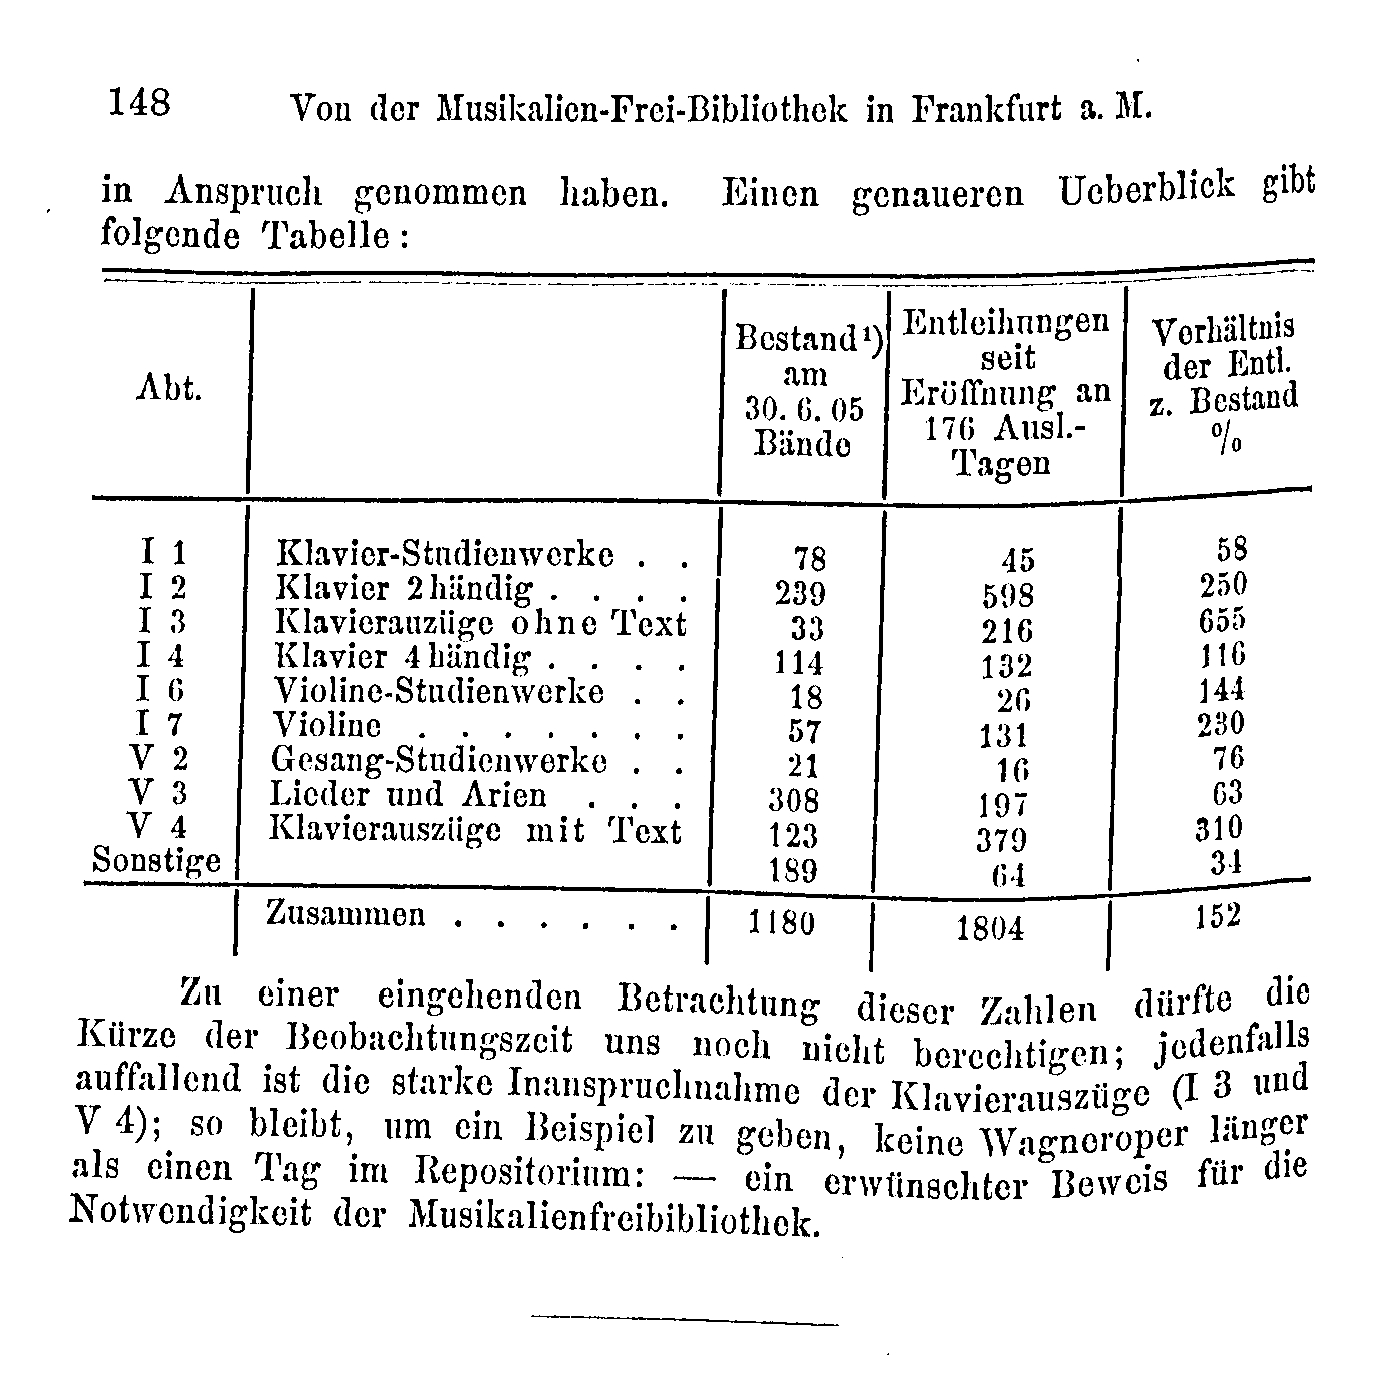
\includegraphics{files/Hanauer_1905.jpg}
\caption{Ausleihstatistik aus Hanauer 1905: 148.}
\end{figure}

Zwei Jahre später, in gewisser Weise als Nachtrag, publizierte Hanauer
dann noch einen Artikel, in welchem er explizit darauf eingeht -- wieder
als mögliches Vorbild für weitere Neugründungen --, wie in Frankfurt am
Main die Musikalien ausgewählt, systematisiert und katalogisiert werden.
(Hanauer 1907) Dabei wird sichtbar, dass man sich in der Bibliothek auf
das, was man heute «ernste Musik» nennen würde, konzentrierte. Populäre
Musik oder Volksmusik wurden nicht beachtet.

Interessant an diesem kurzen Text ist vor allem, dass er in gewisser
Weise nebenher weitere existierende Musikbüchereien erwähnt, die alle in
Grosststädten angesiedelt waren: In München, in Wien und in Paris.

\hypertarget{gegen-musikalischen-schund-1911}{%
\subsection{2.3 Gegen musikalischen Schund
(1911)}\label{gegen-musikalischen-schund-1911}}

Volksbüchereien wurden Anfang des 20. Jahrhunderts als
Erziehungseinrichtungen gegründet. Die genauen Ziele der Büchereien
unterschieden sich je nach Richtung der Träger -- also der Vereine,
politischen Bewegungen und so weiter. Aber ein Thema, das alle umtrieb,
war die Vorstellung, dass es «literarischen Schund» gäbe, der einen
schlechten Einfluss auf die Leser*innen hätte. Was genau als Schund zu
definieren wäre und was genau die wahrgenommenen Gefahren waren,
unterschied sich wieder zwischen den verschiedenen Bewegungen. Aber
woran es keine Zweifel zu geben schien, war, dass es diesen Schund gäbe.

In seinem Artikel zur «Verleihung von Musikalien durch Volksbüchereien»
von 1911 ging es dem Autor Hans Rothhardt nun vor allem darum, zu
diskutieren, ob es analog zum literarischen auch musikalischen Schund
gäbe sowie, ob dagegen die Verleihung von guten Musikalien helfen würde.
Er bejaht beides und plädiert dann dafür, diese guten Musikalien in die
Volksbüchereien aufzunehmen.

Zuerst stellt er fest, dass es keine neue Idee wäre, Noten im
Büchereibestand zu führen. Dafür gäbe es, zumeist in grossen Städten,
schon Vorbilder: «Die Frage, ob überhaupt ein Bedürfnis in weiten
Kreisen der Gesamtbevölkerung für die Verleihung von Musikalien
vorhanden ist, darf wohl ganz unbedenklich bejaht werden.» (Rothhardt
1911: 133)

Zu der Frage, was «musikalische Schundliteratur» sei, gibt er eine in
diesem Diskurs typische Antwort: Einerseits geht er davon aus, dass es
sie gibt, andererseits deutet er recht ungenau an, was genau darunter zu
verstehen sei:

\begin{quote}
«Ja! Es gibt eine musikalische Schundliteratur! Auf sie, als auf einen
Schädling der Allgemeinheit energisch hingewiesen zu haben, ist das
unbestrittene Verdienst des V. Musikpädagogischen Kongresses, der zu
Beginn der Karwoche d.J. {[}das ist die Woche vor Ostern 1911{]} in
Berlin versammelt war. Auf diesem Kongreß hat ein Thema: ‹Die Bekämpfung
der musikalischen Schundliteratur› zur Beratung gestanden und lebhafte
Anteilnahme erweckt. {[}\ldots{]}

Es dürfte hier zu weit führen, zu untersuchen, ob es wirklich eine
musikalische Schundliteratur gibt, wo sie zu finden ist und ob sie in
dem Maße schädlich auf das Volksganze einwirkt, dass sich eine
zielbewußter energischer Kampf dagegen lohnt. Ich will nur auf die
schlüpfrigen Kuplets, auf die üble, zur Sinnlichkeit aufreizende Musik
unserer Tingeltangel und Nachtcafés hinweisen, um leise anzudeuten, in
welcher Richtung die Schäden zu suchen sind. Begnügen wir uns
einstweilen damit, dass die von Eingeweihten erkannten Schäden
tatsächlich vorhanden sind, und dass ihre Bekämpfung einen nicht
unwesentlichen Faktor zur sittlichen Gesundhaltung unseres Volkes und
daraus sich ergebend zu seiner seelischen Veredlung und Höherführung
darstellt.» (Rothhardt 1911: 134)
\end{quote}

Was aus diesen Worten spricht, wenn man sie heute liest, ist einerseits
eine Angst vor einer sich wandelnden, modernisierenden Gesellschaft,
inklusive eines Wandels der Mediennutzung und andererseits eine
Hochschätzung von Musik. Auf der einen Seite würde «Schundmusik» in den
«Nachtcafés» -- die hier als Symbol für die moderne Gesellschaft gelesen
werden können, die mehr Freizeit, Individualisierung, Urbanisierung und
Verbreitung von Technologie repräsentieren -- «das Volk» bedrohen wie
eine Krankheit. Dabei muss «Volk» nicht einmal mit nationalistischer
Bedeutung gelesen werden, sondern kann auch die Angst eines
Mittelschichtangehörigen vor der erhöhten Sichtbarkeit der «unteren
Klassen» in der sich entwickelnden Massengesellschaft
darstellen.\footnote{Es ist nicht ganz eindeutig zu klären, wer der
  Autor ist. Aber zu vermuten ist, dass er identisch mit dem
  Schriftsteller und späteren Bibliothekar in Berlin-Steglitz mit
  gleichem Namen ist. (Vergleiche den Bericht zum fünfjährigen Bestehen
  dieser Bücherei als Gemeindeeinrichtung, in welchem der Autor, Leiter
  der Bücherei, erwähnt, zuvor bei der Volksbücherei in Charlottenburg
  tätig gewesen zu sein, Rothhardt 1926: 2.) Als Schriftsteller
  publizierte er beispielsweise 1923 (in einer nummerierten Auflage von
  200 Stück, also wohl eher als Privatdruck zu bezeichnen) die
  Gedichtsammlung «Musikgärtlein», in der sich ganz explizit auf die
  Oper und Hausmusik sowie «grosse Komponisten» bezogen wird. (Die Titel
  einiger Gedichte lauten: «Trauermarsch aus der Eroica», «Kammermusik»,
  «An mein Cello», «Beethoven», «Beethoven spielt im
  Schwarzspanierhaus», «Beethoven im Himmel», «Mozarts Begräbnis») Auch
  andere seiner Gedichtbände enthalten viele ähnliche Anspielungen.
  (Siehe Rothhardt 1909) Insoweit scheint es nicht zu weit hergeholt,
  ihn einerseits mit dem Autor des hier besprochenen Artikels zu
  identifizieren und in ihm andererseits einen Angehörigen des
  aufstrebenden Bürgertums zu sehen.} Auf der anderen Seite wäre Musik
so besonders, dass sie als eigenes Thema behandelt werden müsse.

Man sollte diese Gedanken und Rhetorik aber nicht als Marotte eines
einzelnen Autors sehen. Er bedient sich eines Diskurses und einer
Darstellung, die sich zeitgenössisch auch in der restlichen Literatur
der Volksbüchereien, der Wissenschaftlichen Bibliotheken oder anderer
Kultureinrichtungen findet. Nicht umsonst kann er auf einen ganzen
«Musikpädagogischen Kongreß» zu diesem Thema verweisen. Was sich hier
zeigt, ist, dass er sich im zeitgenössischen Denken bewegt. Dies gilt
auch für seinen Schluss, in welchem er die Erziehungsaufgabe der
Volksbüchereien auf die Musikalien überträgt. So, wie die Bücherei zum
richtigen Lesen der richtigen Literatur erziehen und dabei von den
Verführungen der modernen Gesellschaft abhalten sollte, gilt diese für
ihn analog für die Musik:

\begin{quote}
«Der unmittelbare Erfolg der Verausgabung von Musikalien in den
Volksbüchereien wird der sein, dass die Bevölkerung namentlich in ihren
mittleren und unteren Schichten an die Pflege guter Musik in Haus und
Familie gewöhnt wird. Die Herz und Geist veredelnde Beschäftigung mit
guter Musik wird einen großen Volksteil, in erster Linie die Jugend, von
andern weniger edlen, ja sogar schädlichen Beschäftigungsarten
ablenken.» (Rothhardt 1911: 135)
\end{quote}

\hypertarget{eine-uxfcbersicht-der-musikbuxfcchereien-1916}{%
\subsection{2.4 Eine Übersicht der Musikbüchereien
(1916)}\label{eine-uxfcbersicht-der-musikbuxfcchereien-1916}}

Eine ganze Anzahl von Jahren erscheint dann zum Thema Musik in der
Literatur der deutschen Volksbüchereien nichts mehr. Das heisst aber
explizit nicht, dass dieses Thema in der Praxis dieser Einrichtungen
irrelevant gewesen wäre, wie dann die nächste Veröffentlichung zeigt.
Der kurze Artikel «Von den Volksbüchereien für Musik» (Marsop 1916),
publiziert und wohl auch schon geschrieben, während der Erste Weltkrieg
stattfand, fasst zusammen, welche eigenständigen, öffentlichen
Musikbüchereien in den letzten Jahren eröffnet worden waren und an
welchen Orten «man mit erfolgreichen Vorbereitungen schon gedeihlich
voran {[}gekommen sei{]}» (Marsop 1916:1) sowie, wo «aussichtsreiche
Verhandlungen im Gange {[}seien{]}» (Marsop 1916:1). Explizit beschränkt
sich der Autor dabei nicht auf Deutschland, sondern zählt zuerst aus der
Schweiz Zürich und aus Österreich-Ungarn Wien, Salzburg, Prag, Brünn,
Graz und Karlsbad auf. Sodann blickt er ins weitere Ausland
(Niederlande) sowie das «feindliche Ausland» mit Italien, Frankreich und
Grossbritannien.

Paul Marsop war in München vor allem als Musikkritiker ansässig, hatte
dort aber auch die Münchener städtische Musikbibliothek gegründet -- die
er im ersten Satz seines Artikels erwähnt -- und scheint deshalb mit den
Entwicklungen der Musikbibliotheken vertraut gewesen zu sein. Ansonsten
erklärt er leider nicht, wie er zu den Informationen gelangte. Insoweit
ist auch nicht klar, ob sie vollständig sind. Was sie aber auch so
zeigen, ist, dass es in den Jahren vor und während des Ersten
Weltkrieges offenbar einige Entwicklungen gegeben hatte. Öffentliche
Musikbibliotheken waren keine Seltenheit mehr, obgleich an seinen
Aufzählungen auch auffällig ist, dass sie vor allem in grossen Städten
zu finden waren oder zumindest angedacht wurden. Relevant ist, dass
diese Musikbibliotheken gegründet wurden, ohne dass dies in der
betreffenden Fachpresse Erwähnung fand. Sie scheinen also schon
einigermassen «Normalität» gewesen zu sein.

\hypertarget{verortung-der-musikbuxfccherei-in-der-musikalischen-erneuerungsbewegung-1927}{%
\subsection{2.5 Verortung der Musikbücherei in der musikalischen
Erneuerungsbewegung
(1927)}\label{verortung-der-musikbuxfccherei-in-der-musikalischen-erneuerungsbewegung-1927}}

Die Jahre der Weimarer Republik waren bekanntlich auch Jahre
verschiedener «Aufbruchsversuche». Nicht nur, dass am Anfang eine
Revolution stand, die von verschiedenen Gruppen mit verschiedenen Zielen
durchgeführt wurde (und für einige von ihnen auch als «nicht beendet»
galt, weswegen es in den frühen Jahren der Weimarer Republik mehrere
Aufstandsversuche gab). Gleichzeitig gab es zahllose andere Ansätze zur
Veränderung des Lebens, ob individuell, gesamtgesellschaftlich oder
künstlerisch. Diese schlossen zum Teil an die Jugend- und
Lebensreformbewegung der Kaiserzeit an, teilweise wurden sie aber auch
als ganz neu verstanden. Sie umfassten zahlreiche Bereiche, von
Ernährungsfragen (Vegetarismus, Alkohol-, Tabak- und Zuckerabstinenz)
über Gesundheits- und Sexualthemen (Freikörperkultur, Sexualaufklärung)
zu gesellschaftlichen Themen (Eugenik, Struktur der internationalen
Staatengemeinschaft). Die Ziele dieser Bewegungen waren widersprüchlich
und liessen auch Zusammenschlüsse zu, die heute absonderlich erscheinen.
Insbesondere die Verbindung von völkischen Vorstellungen und Eugenik mit
vegetarischer, gesundheitsorientierter Lebensweise, die sich in vielen
diese Gruppen (am bekanntesten wohl in der «Vegetarischen
Gartenbaukolonie Eden» in Oranienburg) fanden, ist aus heutigem Blick
erstaunlich. Aber auch, dass sowohl links-revolutionäre, demokratisch
orientierte als auch völkische Bewegungen auf ähnliche Aktivitäten
setzten, um ihre Ziele zu erreichen, war für die damalige Zeit
bezeichnend. (Michalzik 2018, Rindlisbacher 2022)

Musik war eines dieser Gebiete, das wohl von allen Bewegungen in diesem
«veränderungsbereiten» Milieu als wichtig angesehen wurde. Was sich in
dieser Zeit etablierte, war das gemeinsame Singen, ob in
Massenveranstaltungen oder in kleineren Gruppen. Auch hierfür hatte es
Vorläufer gegeben -- beispielsweise die Wandervögelgruppen der
Kaiserzeit, die beim Wandern ständig sangen --, aber in den
1920er-Jahren wurde es zu einem Massenphänomen. Bekannt sind dabei die
Arbeitersingebewegung, gerade im «Roten Wien» der damaligen Zeit (Seidl
1989, Pfoser 1980), und die «Jugendmusikbewegung», die zum Teil von
demokratisch gesinnten, zum Teil von explizit antidemokratisch gesinnten
Akteur*innen vorangetrieben wurde. (Holz 2019, vergleiche auch das
betreffende Kapitel zur Jugendmusikbewegung bei Meier 2022: 184--256) In
letzter sollte das gemeinsame Singen dazu dienen, dass sich Menschen aus
ganz verschiedenen Schichten treffen und sich durch diese kollektive
Aktivität zu einer Gemeinschaft finden könnten. Einer der bekanntesten
Akteure dieser Bewegung war Fritz Jöde, Dozent an der \emph{Staatlichen
Akademien für Kirchen- und Schulmusik} in
Berlin-Charlottenburg\footnote{Charlottenburg war bis zum sogenannten
  «Groß-Berlin Gesetz» von 1920 eine eigenständige Stadt. Wie viele 1920
  nach Berlin eingegliederte Gemeinden behielt sie eine gewisse eigene
  Identität bei, die teilweise auch heute noch baulich sichtbar ist.
  Deshalb wird sie in diesem Text mit dem damals auch verbreiteten
  Doppelname geführt. Seit 2001 ist sie Teil des Berliner Stadtbezirks
  Charlottenburg-Wilmersdorf.} sowie einer der effektivsten Umsetzer der
sogenannten Kestenbergschen Reformen (Mahlert 2008, Richter 2008),
welche während der Weimarer Republik den Musikunterricht in Schulen
zeitgenössisch ausrichteten, den Musikunterricht ausserhalb von Schulen,
inklusive der Ausbildung der ausserschulischen Lehrkräfte, vorantrieben
und auf eine Demokratisierung des Zugangs zu Musik zielten.\footnote{Eschen
  2008, Holz 2019. Vergleiche für eine zusammenfassende Darstellung auch
  das betreffende Kapitel bei Stoverock 2013, auch wenn Jödes Arbeit in
  dieser Studie nicht im Fokus steht.} Jöde organisierte in
Berlin-Charlottenburg ab 1923 auch die erste staatliche
Jugendmusikschule im DACH-Raum, etablierte ab 1926 «offene
Singestunden», bei denen teilweise hunderte Personen zusammenkamen und
experimentierte mit solchen Singestunden auch im damals neuen
Rundfunk.\footnote{Vergleiche die betreffenden Kapitel bei Holz 2019:
  123--144 und Holz 2019: 145--161.}

Relevant ist dies alles für einen Artikel, welcher 1927 in der
Zeitschrift \emph{Hefte für Büchereiwesen} erschien. Der Artikel besteht
aus zwei Teilen, einer Einleitung von Walter Hofmann -- einem der
umtriebigsten Bibliothekar*innen der 1910er- bis 1930er-Jahre und unter
anderem Leiter der \emph{Stadtbibliothek Leipzig} -- und dem
eigentlichen Text von Konrad Ameln, dem «Musikreferenten» der
\emph{Stadtbibliothek Leipzig}. Die Stadtbibliothek unter Hofmann nahm
damals für sich in Anspruch, Vorreiter einer neuen, zeitgemässen
Büchereiarbeit zu sein. In diesem Rahmen ist dieser Artikel zu lesen.
Hofmann verortet die moderne Musikbücherei in der «musikalischen
Erneuerungsbewegung», die er unter anderem mit Jöde -- also vor allem
ihrem demokratisch orientierten Teil -- identifiziert. Diese würde
anstreben, die Musik «aus den Fesseln spezialistischer Fachforschung und
artistischen Virtuosentums {[}zu{]} befreien» (Hofmann \& Ameln 1927:
71) und sei «so allen ähnlichen Bestrebungen und Fragestellungen in der
freien Volksbildung eng verwandt» (Hofmann \& Ameln 1927: 71). Mit
freier Volksbildung meinte Hofmann meist die Volksbüchereien nach dem
Vorbild der Leipziger Stadtbibliothek, aber auch die Teile der weiteren
Erwachsenenbildung, die sich nicht einer politischen Richtung
zuordneten. «Durch diese Musikbewegung ist deutlich geworden, daß auch
in der freien Volksbildungsarbeit der Musik und vor allem der
Musikausübung der Laien eine erhöhte Bedeutung zukommt.» (Hofmann \&
Ameln 1927: 71) Aufgabe der Volksbücherei sei es jetzt, diese
Erneuerungsbewegung zu unterstützen. Bisher sei dies nicht geschehen,
sondern «{[}w{]}enn die volkstümliche Bücherei bisher sich überhaupt mit
der ‹Musik› befaßte, dann geschah dies bisher in erster Linie dadurch,
daß in größerem oder geringerem Umfange Literatur \emph{über} Musik,
musikgeschichtliche, musikästhetische, musikpädagogische Werke,
Musikerbiographien, Werke zur Instrumentenlehre u. a. eingestellt
wurden.» (Hofmann \& Ameln 1927: 72) Hofmann plädiert nun dafür, dass
die Büchereien die Anforderungen der neuen Bewegung in den Mittelpunkt
ihrer Arbeit stellen sollten, aber ohne die bisherige Fokussierung
aufzugeben, denn «{[}e{]}ine solche Einseitigkeit würde der deutschen
Volksbüchereibewegung schlecht stehen.» (Hofmann \& Ameln 1927: 72) Er
lässt die konkrete Aufgabe also auch etwas im Ungefähren. Zwar betont
er, dass die Büchereiarbeit planmässig und geordnet erfolgen solle, dass
eine Auswahl nötig sei und so weiter. Aber grundsätzlich lässt er dann
vieles als für die Volksbücherei passende Literatur gelten. Allerdings
kündigt er an, dass die Musik in den von ihm verantworteten \emph{Hefte
für Büchereiwesen} in Zukunft einen grösseren Platz einnehmen
würde.\footnote{Das passierte dann nicht wirklich, wobei bemerkt werden
  muss, dass die \emph{Hefte} recht unregelmässig erschienen und Hofmann
  recht oft Pläne entwarf, die er dann doch nicht in dem Masse umsetzen
  konnte, wie von ihm konzipiert.}

Anschliessend übernimmt Ameln, der in seinem Teil des Textes
grundsätzlich die gleichen Aussagen macht. Er stellt zuerst fest, dass
die Musik in den deutschen Volksbüchereien «ein Stiefkind» (Hofmann \&
Ameln 1927: 74) sei, allerdings aus strukturellen Gründen. Für eine gut
geführte Musikbücherei bedürfe es eines besonderen Personals, das sich
neben der bibliothekarischen Ausbildung auch mit Musik und
Musikliteratur auskennen müsse. Dieses sei schwer zu finden. Zudem wären
die meisten Musikbüchereien eigenständig und nicht direkt an eine
Volksbücherei angebunden. Es fällt auf, dass er dies als Status quo
benennt, aber ohne klarzumachen, woher er diese Kenntnisse hat.
Eventuell schildert er hier also seinen Eindruck, aber nicht den
tatsächlichen Stand.

Weiterhin postuliert er, dass die Musik ihren gesellschaftlichen Werte
verloren hätte («Nur in wenigen Kreisen hat sich eine Vorstellung von
dem überpersönlichen Wert der Musik erhalten, von ihrer
\emph{erzieherischen, bildenden, bindenden} Kraft, die in älterer Zeit
noch hoch geschätzt wurde.» (Hofmann \& Ameln 1927: 74)), erst in
jüngerer Zeit hätte «die Jugend» ihre Bedeutung wieder entdeckt. Solche
Diskurse des Niedergangs, nicht nur, aber auch der Musik, sowie ihrer
Wiederentdeckung durch «die Jugend» (die hier eher für Lebensreform- und
ähnliche Bewegungen stand und nicht unbedingt auf ein Lebensalter
festgelegt war), waren in dieser Zeit normal. Gerade auch in der
«musikalischen Erneuerungsbewegung» wurden sie oft reproduziert, wobei
es aus heutiger Sicht eher erscheint, als hätte sich die Bedeutung von
Musik unter anderem durch die beginnende Demokratisierung der
Gesellschaft sowie die kapitalistische Unterhaltungskultur geändert.
(Holz 2019) In diesem Sinne war die Beschäftigung der Jugend- und
Lebensreformbewegung wohl weniger die «Wiederentdeckung» einer
vergessenen Tradition, als vielmehr eine moderne Reaktion auf die sich
verändernde Gesellschaft. Relevant ist aber, dass Ameln die
Diskursfiguren der Bewegungen übernimmt und mit den Ansprüchen auf eine
geplante, auf Erziehungsziele ausgerichtete Büchereiarbeit verbindet,
wie sie in der damaligen Zeit unter anderem in Leipzig propagiert
wurden.

Er plädiert dafür, gesonderte bibliothekarische Literatur zum Thema zu
erarbeiten und herauszugeben. Dabei denkt er offenbar vor allem an
Besprechungen -- wie sie auch für Belletristik normal waren -- in der
\emph{Hefte für Büchereiwesen} selber, aber auch an weitere
Handreichungen. («So wird es notwendig sein, erst einmal eine Art
Grundstock, einen Idealbestand auszuwählen, in einer Bücherei
aufzubauen, bei seiner Vermittlung Erfahrungen sammeln und diese den
daran interessierten Büchereileitern und Bibliothekaren zugänglich zu
machen.» (Hofmann \& Ameln 1927: 78)) Kurz gesagt wollte er die gleiche
Arbeitsweise, wie sie in Leipzig auch für andere Bereiche des
Volksbüchereiwesens angewandt wurde, auf die Musikabteilung übertragen
wissen. Das Hauptaugenmerk sollte dabei auf Noten liegen; die Literatur
über Musik erst an zweiter Stelle stehen. Nicht die Fachleute, sondern
die musizier- und singebegeisterten Personen sollten im Fokus dieses
Bestandsaufbaus stehen.

\hypertarget{schallplatten-bildungspflege-und-hausmusik-1930}{%
\subsection{2.6 Schallplatten, Bildungspflege und Hausmusik
(1930)}\label{schallplatten-bildungspflege-und-hausmusik-1930}}

Innerhalb der deutschsprachigen Volksbüchereibewegung -- aber nicht der
anderen Büchereien, also den Arbeiterbibliotheken, den katholischen
Bibliotheken oder den gewerblichen Leihbibliotheken -- fand ab den
1920ern bis in die Zeit des Nationalsozialismus hinein der sogenannte
«Richtungsstreit» statt.\footnote{Das gilt auch für die weitere
  Erwachsenenbildung, also zum Beispiel die Volkshochschulen, bei denen
  dieser Streit zeitgleich, mit den gleichen Argumenten und
  Begrifflichkeiten, zum Teil auch unter Beteiligung der gleichen
  Akteur*innen, stattfand. (Pögeller 1974)} In ihm ging es um die
Stellung und Aufgabe der Büchereien sowie die Frage, wie und wozu
Menschen durch die Büchereien erzogen werden sollten. Beide Gruppen, die
diesen Streit ausfochten, verstanden die Büchereien als Teil der
«Bildungspflege», also als Bildungseinrichtungen, die vor allem nach der
Schul- und Ausbildungszeit Menschen erreichen sollten, wobei beide
Seiten auch die gesamte Gesellschaft im Blick hatten und Menschen aus
allen Schichten ansprechen wollten. Beide sahen diese Aufgabe in einer
aktiven «Pflege», also Erziehung, nicht in einem reinen zur Verfügung
stellen von Medien zur selbstbestimmten Bildung. Diskutiert wurde eher,
welche Menschen (Eher wenige, herausragende Personen oder eher viele?)
wie erreicht werden könnten, welche büchereitechnischen Mittel dafür
angewandt oder auch, ob und wie Veranstaltungen der Bildungspflege in
Volksbüchereien gestaltet werden sollten.

Dieser Kontext ist nun für den Artikel relevant, den Erwin Ackerknecht
1930 unter dem Titel «Bildungspflege und Schallplatte» (Ackerknecht
1930) publizierte. Ackerknecht war nämlich einer der Protagonist*innen
dieses «Richtungsstreits». Auch wenn er es selber abstritt, war er --
als einer der publikationsstärksten Bibliothekar*innen seiner Zeit --
einer der Hauptvertreter der «Stettiner Richtung» (nach der Stadt, in
welcher er damals gleichzeitig die Stadtbibliothek und die
Volkshochschule führte). Die andere Richtung, oft «Leipziger Richtung»
genannt (nach dem Wirkungsort von Walter Hofmann) hatte mit \emph{Hefte
für Büchereiwesen} und dem \emph{Volksbildungsarchiv} ihre eigenen
Publikationsorgane. Aus diesen stammte der hier zuvor besprochene
Artikel. Was damit sichtbar wird, ist, dass dieser Richtungsstreit --
welcher damals tatsächlich mit harten Bandagen geführt wurde -- keinen
Einfluss darauf hatte, ob in Volksbüchereien Musik als relevantes Thema
angesehen wurde. Vielmehr fühlten beide Seiten die Notwendigkeit, sich
mit ihr auseinanderzusetzen. Darüber hinaus weist der Artikel selber
ganz am Ende (Ackerknecht 1930: 13ff.) darauf hin, dass auch die
katholischen Büchereien (siehe zum Beispiel Zoumer 1931) sich intensiv
mit Fragen von Schallplatten, Musik, Radio und Bildungspflege befassen
würden. (Wir können also vermuten, auch wenn es nicht in der Literatur
sichtbar war, dass sich ebenso die Arbeiterbibliotheken mit dem Thema
befassten.)

Aber zurück zum eigentlichen Artikel. Ausgangspunkt ist für Ackerknecht
die Frage, «wie weit sich die Schallplatte in den Dienst der
Bildungspflege stellen lasse» (Ackerknecht 1930: 7). Er sieht die
technische Entwicklung so weit fortgeschritten, «daß ein wirklicher
musikalischer Genuß auch für den Feinhörigen gewährleistet werden kann»
(Ackerknecht 1930: 7). Es sei deshalb Zeit, sich zu fragen, wie sie für
die Bildungsarbeit in Büchereien -- und auch, weil dies für Ackerknecht
immer zusammengehörte, Volkshochschulen -- genutzt werden könne. Dabei
unterteilt er: Schallplatten könnten einerseits einen Gesamteindruck von
Musikstücken vermitteln («Stimmungswirkung», Ackerknecht 1930: 8) und
andererseits als Material für Bildungsveranstaltungen, bei denen auch
erläutert und gelernt wird, genutzt werden («Bildungswirkung»,
Ackerknecht 1930: 8). Insbesondere hebt er hervor, dass man ein
Musikstück von einer Schallplatte auch mehrfach abspielen könne.
Allerdings, und dies prägte die Texte von Ackerknecht, warnt er davor,
praktisch zu viel auf einmal lehren zu wollen. Bildungspflege hiesse
nicht, Musikanalyse lehren. Es gehe um Einführungen, Übersichten oder
auch die Vor- und Nachbereitung von Opernbesuchen. (Ackerknecht 1930: 8)
Dies fügt sich ein in die Arbeit von Volksbüchereien, die Ackerknecht
unter Bildungspflege versteht -- Kurse, durchgeplante Vorleseabende oder
auch gemeinsame Besuche von anderen Einrichtungen wie Museen, Galerien
oder halt Opern, die in kleinen, von der Bibliothek organisierten
Gruppen vorgenommen würden. (Ackerknecht 1924) Für diese «freilich
{[}fände man{]} in der Schallplatte ein unvergleichliches
Anschauungsmaterial» (Ackerknecht 1930: 8).

Zudem postuliert Ackerknecht, dass sich die Schallplatte als Medium
durchsetzen würde, während die «Hausmusik» (Ackerknecht 1930: 9), also
das Musikmachen daheim, im Rückgang begriffen wäre. Auch dies war ein
zeitgenössischer Diskurs: Ständig wurde behauptet -- ohne das in Zahlen
auszudrücken --, dass immer seltener Hausmusik gemacht würde, was als
Problem der Moderne angesehen wurde. Ackerknecht scheint es in diesem
Text als Faktum zu begreifen, dass er zwar bedauert (Ackerknecht 1930:
9), aber auch nicht aufhalten will. Er betont aber, dass auch «dem immer
kleiner werdenden Häuflein der Hausmusikanten durch öffentliche
Musikalienbüchereien» (Ackerknecht 1930: 9) Noten zur Verfügung gestellt
werden müssten. Diese will er also nicht durch Schallplatten ersetzen.

Zu der eigentlichen Frage, nämlich wie Schallplatten in der
Bildungspflege eingesetzt werden sollten, betont er zuerst, dass mit
ihnen «{[}e{]}ine außerordentliche Erweiterung {[}des{]} musikalischen
und zugleich völkerpsychologischen Horizontes {[}der
Vortragsveranstaltungen in den Volksbüchereien{]} durch die
fremdländische Musik {[}möglich{]} werden». (Ackerknecht 1930: 10) Es
geht also um Horizonterweiterung. Gleichzeitig betont er, dass alle
diese Veranstaltungen gut geplant und nicht zu lang oder spezifisch sein
dürften. Musik solle, wie gesagt, nicht analysiert, sondern für die
richtige Stimmung genutzt werden -- also vor allem als Ergänzung des
Gesagten. (Ackerknecht 1930: 11)

\hypertarget{die-aufgaben-der-modernen-musikbuxfccherei-1931}{%
\subsection{2.7 Die Aufgaben der modernen Musikbücherei
(1931)}\label{die-aufgaben-der-modernen-musikbuxfccherei-1931}}

Aus der heutigen Sicht scheinen die frühen 1930er-Jahre, gerade in
Deutschland, eine Zeit gewesen zu sein, die mehr oder minder auf die
Katastrophe des Nationalsozialismus zulief. Das aber war in diesen
Jahren nicht unbedingt ausgemacht -- immer waren zeitgenössisch auch
andere Entwicklungen denkbar. Sichtbar war damals allerdings, dass die
Zeit geprägt war durch grosse Verwerfungen -- die wir heute vor allem
als Entwicklungen der technischen und gesellschaftlichen Modernisierung
ansehen würden --, von Versuchen, diese Verwerfungen zu verstehen und zu
steuern sowie vielen Versuchen, gesellschaftlich einen übergreifenden
Zusammenhalt herzustellen, welcher diese Verwerfungen wieder auffangen
würde. Das galt nicht nur für den Nationalsozialismus, der sich mit
seiner Vorstellung der «Volksgemeinschaft» (inklusive der Ausschlüsse
aus dieser) an dieser Suche beteiligte, sondern für ganz
unterschiedliche Bewegungen. Es war eher eine verbreitete Zeitanalyse,
der gleichzeitig immer auch widersprochen wurde. Wichtig hier ist, dass
der Musik und dem gemeinsamen Singen dabei oft eine Rolle bei der Suche
nach solch einem übergreifenden Zusammenhalt zugesprochen wurde. Das ist
ein Grund, warum dann während des Nationalsozialismus dem Singen ein
grosser Stellenwert eingeräumt wurde (Niesen 1999). Aber, wie schon
dargestellt, auch die bündische Jugend, der Wandervogel oder aber die
Arbeitersingegruppen des Austromarxismus griffen auf die vorgeblich
vereinende Macht des Singens zurück.

In diesem Kontext muss man den letzten Artikel lesen, der sich in der
Weimarer Republik mit dem Zusammenhang von Volksbücherei und Musik
befasste. Im Gegensatz zu anderen hier vorgestellten Texten, die sich
oft um Objektivität bemühen, ist dieser voller Pathos. Als Beispiel sei
der erste Absatz zitiert:

\begin{quote}
«Hat man in jüngster Zeit eine ‹Entgötterung› der Musik, eine
Mechanisierung und Maschinisierung dieses irrationalsten aller
menschlichen Schaffens- und Erlebnisgebiete feststellen zu müssen
geglaubt -- teilweise vielleicht nicht mit Unrecht --, so kann doch
darüber kein Zweifel bestehen, dass wir heute eine Renaissance aller
musikalischen Urkräfte erleben, die allen im Dienste der Bildungspflege
Stehenden neue wichtige Aufgaben stellt. Musik gilt heute nicht mehr nur
als eine ästhetische Angelegenheit begüterter Kreise oder als Schmuck
und Genuß des Lebens für besondere Feier- und Feststunden, sondern sie
gehört heute dem ganzen Volke als ein nicht zu entbehrender Bestandteil
seines Lebens, als eine seelische Notwendigkeit seines Alltags, sie ist
unentbehrlich geworden zur Wiedergewinnung der uns durch übergroße
Differenzierung verlorengegangenen geistig-seelischen Totalität. Damit
ist die Musik wie keine andere der Künste berufen, sowohl zu einer
inneren Erneuerung des \emph{Einzelmenschen} zu verhelfen wie den
inneren Zusammenhang des \emph{Volksganzen} zu stärken. So kommt ihr
gerade gegenwärtig wieder eine zentrale Stellung im geistigen Haushalt
der Nation zu.» (Bayer 1931: 176)
\end{quote}

Der Autor, Karl Bayer, postuliert dann weiter, dass es die Aufgabe der
Volksbüchereien wäre, Musik in der Bildungspflege einzusetzen. Dabei hat
er explizit nationalistische Argumente. Musik und Bildung zur Musik
sollten Deutschland einen Platz in der Welt wieder erobern, den es
einmal gehabt hätte: «Es darf als eine der vornehmsten Aufgaben aller
behördlichen Stellen, die es angeht, bezeichnet werden, daran zu
arbeiten, daß unsere Nation diese Weltgeltung auf dem Wege der
friedlichen Eroberung sich wiedererringe» (Bayer 1931: 179). So schreibt
er zum Beispiel auch nicht einfach von Berlin, sondern von «unserer
Reichshauptstadt und größten Bibliotheksstadt, die zugleich wohl die
erste Musikstadt der Welt ist oder doch bisher gewesen ist und weiter
sein soll» (Bayer 1931: 177). Zudem postuliert er -- im Gegensatz zu
dem, was bislang in diesem Artikel hier sichtbar wurde -- dass es das
«auch gerade in bibliothekarischen Kreisen immer noch verbreitete
Vorurteil {[}gäbe{]}, Musikalien gehörten nicht in die Bibliotheken»
(Bayer 1931: 179), welches zu beseitigen wäre.\footnote{Man muss solche
  allgemeinen Aussagen auch als rhetorisches Mittel interpretieren.
  Immerhin konnte der Autor seinen Text, trotz dieses Vorwurfs,
  unwidersprochen in einer Volksbüchereizeitschrift veröffentlichen.}

Grundsätzlich fordert Bayer mehr Musikbibliotheken für die allgemeine
Öffentlichkeit. Es gäbe viel zu wenige und auch diese seien unzureichend
ausgestattet. («Schon eine kurze Umschau ergibt, dass auf diesem Gebiete
fast alles noch zu tun ist.» (Bayer 1931: 177.)) Sie sollten in
«Zentralbibliotheken» organisiert sein -- Abteilungen in
Volksbüchereien, die dann langsam zu eigenständigen Musikbibliotheken
ausgebaut würden. Daneben solle es weiter kleinere Musikbüchereien
geben. Wichtig ist ihm, dass diese Bibliotheken einen Bildungsauftrag
hätten. Sie sollten zum Musikmachen erziehen und gerade keine Musik zu
Unterhaltungszwecken bereitstellen: «{[}M{]}aßgebend für die
Anschaffungspolitik {[}ist{]} also der erziehliche {[}sic!{]} und
bildende Charakter der Sammlung{[}.{]} Damit scheiden alle lediglich dem
Unterhaltungsbedürfnis im platten Sinne dienenden und alle taggebundenen
Werke von vornherein aus {[}\ldots{]}; ferner werden Werke
zeitgenössischer Komponisten, soweit deren Bedeutung noch sehr
umstritten ist, nur nach eingehender Prüfung von Fall zu Fall
eingestellt werden dürfen{[}.{]}» (Bayer 1931: 180) Diese Kriterien
erscheinen heute nicht nur überspitzt, sondern auch gänzlich unmöglich
umzusetzen -- sie würden eine Prüfung aller eingestellten Medien nach
Kriterien, die schwerlich objektivierbar sind, bedeuten. Aber sie waren
für Volksbüchereien der damaligen Zeit nicht so abwegig. Auch für Bücher
wurden ähnliche Kriterien gefordert und auch angelegt. (Das ist ein
Grund, warum die Bestände der Volksbüchereien weit kleiner waren, als
die der heutigen Öffentlichen Bibliotheken.) Insoweit bewegt sich Bayer
hier, wenn auch etwas überspannt, im zeitgenössischen bibliothekarischen
Diskurs.

Im Anschluss geht Bayer einige Werke durch, die er als besonders
empfehlenswert für Musikbüchereien ansieht. Zudem entwirft er gleich ein
umfassendes Programm für ausgebaute Musikbüchereien. Sie sollten eigene
Musiksäle oder Musikzimmer (schalldicht und gegebenenfalls mit
Instrumenten sowie Anschlüssen für Radioempfang und -übertragung)
erhalten. Eigene Jugendabteilungen seien zu empfehlen, ebenso eine
«Schallplatten-Bibliothek» (Bayer 1931: 182). Nicht zuletzt sollten die
Büchereien eigene Konzerte anbieten, um Geld einzunehmen, aber auch, um
für die Bücherei und ihre Angebote zu werben. (Bayer 1931: 184)
Gleichzeitig fordert er, dass diese Einrichtungen von gesondert
ausgebildeten «Beamten der Musikalienausleihe» (Bayer 1931: 184) geführt
würden, welche sich Kenntnisse der Notenliteratur aneignen müssten,
vergleichbar mit denen, wie sie Bibliothekar*innen sonst über Bücher
hätten.

Was neben dem Pathos und nationalistischen Einschlag dieses Textes
auffällt, ist, dass der Autor hier vor allem ein aufgebautes
Musikbibliothekssystem entwirft, inklusive Aufgabe und
Veranstaltungsarbeit, ohne sich offenbar darüber Gedanken zu machen, wie
dieses konkret entstehen (und finanziert) werden sollte.

\hypertarget{nationalsozialismus}{%
\section{3. Nationalsozialismus}\label{nationalsozialismus}}

Die Beiträge zu Musik und Volksbüchereien, welche während des
Nationalsozialismus erschienen, lassen sich in zwei Gruppen
zusammenfassen: Während in den ersten Jahren des Regimes keine Texte
erschienen, änderte sich dies 1937. Dann erschienen wieder -- das ist
die erste Gruppe -- längere Beiträge, die sich auch mit grundsätzlichen
Fragen der Musikbüchereien befassten. Nachdem das Regime 1939 den
Zweiten Weltkrieg begonnen hatte, änderten sich -- das ist dann die
zweite Gruppe -- diese Texte. Nicht nur wurden sie kürzer, was sich
teilweise mit den verfügbaren Papier- und Druckressourcen erklären
lässt. Sie konzentrierten sich auch auf die konkrete Arbeit der
Einrichtungen. Während des Krieges erschienen, wenn man sie so nennen
will, viele Praxisbeiträge, die sich nicht mehr damit aufhielten,
grundsätzliche Fragen zu klären. In gewisser Weise scheint in diesen
Beiträgen durch, dass sich Musikbüchereien als ein Büchereityp etabliert
hatten.

Wieder ist dies in die zeitgenössische Entwicklung einzubetten. (Klause
2021, Zapke 2020, Holz 2019: 201--260, Petit 2018, Stoverock 2013,
Nierenz 2010, Niessen 1999) Was an den im Folgenden vorgestellten Texten
auffällt, ist, dass sie sich positiv auf die nationalsozialistische
Ideologie beziehen, während gleichzeitig die Verbrechen des Regimes gar
nicht angesprochen werden. Beispielsweise wird der Ausschluss von
jüdischen Musiker*innen und Leser*innen nicht angesprochen -- dafür
fehlen allerdings auch meist direkte antisemitische Invektiven. Ebenso
wird zum Beispiel nicht darauf eingegangen, dass Menschen mit
Behinderungen aus dem Alltag ausgeschlossen und getötet worden waren.
Vielmehr wird sich kontinuierlich affirmativ auf das «deutsche Volk» und
die «deutsche Musik» bezogen. (Die Vorstellung von Ackerknecht (1930),
dass Musik den Horizont erweitern würde, gibt es in ihnen nicht mehr;
vielmehr geht es gerade darum, praktisch keine Musik aus anderen Ländern
zu hören.)

Gleichzeitig finden sich in den folgend vorgestellten Texten zwei
Photostrecken neuer Musikbüchereien. Dies passte ebenso zur Zeit. Zum
einen verstand sich der Nationalsozialismus als modernes,
fortschrittliches Regime, welches explizit auf technische Entwicklungen
setzte. Dazu gehörte auch der verstärkte Einsatz von Fotografie -- eine
Entwicklung, die allerdings schon in den 1920er-Jahren eingesetzt hatte
und die sich nicht nur in der bibliothekarischen Literatur zeigte. Zum
anderen postulierte der nationalsozialistische Staat unter anderem die
Hoheit über das Volksbüchereiwesen -- es sollte zur allgemeinen Aufgabe
von Staat und Gemeinden werden, die zentral gesteuert, dafür dann aber
auch landesweit garantiert würden. Dies wurde als Teil der
«Volksgemeinschaft» angesehen. Dafür wurden im Volksbüchereiwesen unter
anderen alle vorhandenen Gruppierungen zusammengeführt und es wurde im
\emph{Reichsministerium für Wissenschaft, Erziehung und Volksbildung}
eine eigene Stelle für das Volksbüchereiwesen geschaffen, die
\emph{Reichsstelle für das Volksbüchereiwesen}. Auch die beiden bis dato
erscheinenden reichsweiten Zeitschriften wurden beendet, damit ab 1934
mit \emph{Die Bücherei: Zeitschrift für Schrifttumspflege} eine neue
Zeitschrift erscheinen konnte. Diese hatte erkennbar mehr Ressourcen zur
Verfügung, als die vorher erscheinenden, was sich auch in den
zahlreichen Bildstrecken zeigte, die es zuvor nicht gab.\footnote{Dies
  heisst auch, dass es von Büchereien im Nationalsozialismus mehr und
  bessere bildliche Darstellungen gibt, als aus den Zeiten zuvor.}

Selbstverständlich: Das nationalsozialistische System war dadurch
gekennzeichnet, dass es ständige Kämpfe zwischen verschiedenen
Fraktionen und Stellen gab, die niemals zu einem Ende geführt
wurden.\footnote{Siehe auch Petit 2020, die das explizit für das Feld
  Musik beschreibt.} Dies gilt auch für das Volksbüchereiwesen: Neben
dem \emph{Reichserziehungsministerium} erhoben auch andere Stellen den
Anspruch, Einfluss auf das Volksbüchereiwesen zu nehmen, beispielsweise
die \emph{Hitlerjugend}, das «Amt Rosenberg» («\emph{Beauftragter des
Führers für die Überwachung der gesamten geistigen und weltanschaulichen
Schulung und Erziehung der NSDAP}») oder das \emph{Reichsministerium für
Volksaufklärung und Propaganda} unter Joseph Goebbels. (Barbian 2010)
Gleichzeitig wurden insbesondere von staatlichen Beratungsstellen im
Laufe der Zeit wieder eigene Zeitschriften herausgegeben, allerdings
offenbar ohne, dass in ihnen Musikbüchereien thematisiert wurden.

Nichtsdestotrotz wurde im Nationalsozialismus ein Programm des «Aufbaus»
von Volksbüchereien und dann auch von spezialisierten Büchereitypen
begonnen. Aufbau ist hier einerseits als Polemik zu verstehen: Es wurde
behauptet, dass zuvor kaum wirkliche Volksbüchereien bestanden hätten,
sondern dass nur durch den Nationalsozialismus eine sinnvolle
Zusammenfassung der Büchereien und eine systematische Planung
vorgenommen werden könnte. Faktisch wurden dann auch viele Büchereien,
die zuvor von Vereinen oder politischen Gruppen geführt wurden,
geschlossen und zusammengeführt. (Einzig die katholischen Bibliotheken
konnten, aufgrund des «Reichskonkordats» zwischen dem Vatikan und
Deutschland von 1933, unter Einschränkung ihrer Aufgaben,
weiterbestehen. (Trippen 1996)) Diese Zusammenführung -- praktisch wohl
oft auch eine Reduzierung des Angebots -- wurde dann als Aufbau nach dem
Prinzip von eher wenigen, dafür zentralen Volksbüchereien in
Verantwortung der jeweiligen Gemeinden beschrieben. Andererseits gab es
aber auch die praktische Seite dieses Aufbaus: Nachdem zuerst
Volksbüchereien geschlossen und zusammengeführt wurden, wurden
anschliessend tatsächlich neue gebaut, modern eingerichtet und,
insbesondere für den Raum ausserhalb der grossen Städte, zentrale
Beratungsstellen eingerichtet oder aber, wo sie schon existierten,
übernommen. Diese Zentralisierung -- die, wie so vieles im
Nationalsozialismus, in weiten Teilen auch Plan blieb -- führte auch
dazu, dass sich nach einigen Jahren dieses Aufbaus in der Literatur
thematisch spezifischen Büchereitypen zugewandt wurde. Dies zeigt sich
auch in der Zeitschrift \emph{Die Bibliothek}. Hier finden sich ab 1937
nämlich nicht nur Beiträge zu Musikbüchereien, sondern zum Beispiel auch
zu Gefängnisbüchereien (Löwe 1938) oder Schulbibliotheken (Schriewer
1938, Heiligenstaedt 1938). Dass während des Nationalsozialismus für
solche Büchereitypen zunehmend spezielle Buchlisten oder -- im Falle der
Musikalien -- gesonderte Katalogisierungsregeln erschienen
(Weiß-Reyscher 1938), gehört zur Geschichte dieses «Aufbaus».

\hypertarget{nochmal-die-aufgabe-der-modernen-musikbuxfccherei-1937}{%
\subsection{3.1 Nochmal: Die Aufgabe der modernen Musikbücherei
(1937)}\label{nochmal-die-aufgabe-der-modernen-musikbuxfccherei-1937}}

Den Auftakt der Publikationen zum Themenfeld, die während des
Nationalsozialismus erschienen, machte ein Text, der wegen seiner Länge
in zwei Teilen erscheinen musste. Trotzdem war er noch gekürzt worden,
worauf die Redaktion explizit hinwies, «{[}d{]}a der Verfasser
befürchtet, daß die Komposition des Ganzen {[}\ldots{]} durch die
Streichungen gelitten hat{[}.{]}» (Angermann 1937b: 301) Oder anders
gesagt, nahm sich der Autor, Rudolf Angermann -- Leiter der
\emph{Stadtbücherei Hagen}, die auch eine Musikbücherei
betrieb\footnote{Ein biografisches Kuriosum ist, dass Angermann zuvor
  noch unter Erwin Ackerknecht in Stettin gearbeitet hatte. Ackerknecht
  hatte, wie weiter oben gezeigt, Musik als Mittel angesehen,
  völkerverständigend zu wirken. Angermann geht, zumindest während des
  Nationalsozialismus, einen ganz anderen Weg.} sowie Vorsitzender des
\emph{Referats Musikbüchereien} der \emph{Reichsstelle für das
Volksbüchereiwesen} im Reichserziehungsministerium -- vor, in diesem nur
«Die Musikbücherei» genannten Text gleich das gesamte Feld zu bearbeiten
-- von der Aufgabenstellung dieser Büchereien bis zu deren konkreter
Arbeit.

Zuerst versucht er zu klären, wofür es überhaupt Musikbüchereien geben
sollte. Dabei geht er explizit von einem Erziehungsauftrag aus. In einem
«natürliche Zustand» würden alle Völker ihre jeweilige Musik haben,
wobei das deutsche «ein hochmusikalisches Volk» (Angermann 1937b: 303)
sei. Allerdings sei es aktuell nicht der Fall, dass im Deutschen Reich
Musik weit verbreitet wäre. Musikerziehung, zu der die Büchereien
gehörten, hätte nun die Aufgabe, das Volk dazu zu bringen, die ihm
zugehörige Musik aktiv zu leben.\footnote{Vergleiche die Darstellung der
  Ziele musikalischer Bildung in der \emph{Hitlerjugend} und dem
  \emph{Bund Deutscher Mädel} bei Stoverock (2013), um zu sehen, dass
  die Position von Angermann nicht singulär war, sondern im Mainstream
  der Verlautbarungen während des Nationalsozialismus, insbesondere zu
  Beginn des Regimes, stand.} Dabei geht es Angermann vor allem um das
Tun, also das Singen und Musizieren, nicht so sehr um Musiktheorie oder
eine vertiefte Reflexion über Musik.

\begin{quote}
«Wie können wir nun den unnatürlichen Zustand beseitigen, der einen
großen Volksteil von einem Reich höchster Menschheitsgüter ausschließt?
Wie können wir Musik wieder volkswirksam, volkläufig machen? -- Wir
gestehen sofort: wir können das von uns aus nicht. Hier liegen höchste
Aufgaben der deutschen Volksführung, hier wirken neuaufbrechende Kräfte
des Volkes selbst das ihre. Wir sind überzeugt, dass Volksmusikerziehung
gelingen kann, wenn die Musik aus dem Nur-Fachlichen herausgelöst,
übertriebene artistische Anforderungen fallen gelassen und vor allem:
der Begriff des Musikalischseins nicht weiter gespannt wird als der
sonstigen Kunstverständnisses, d.h. beschränkt wird auf \emph{die
Fähigkeit musikalische Gestalten in ihrer vollen und tiefen Wirklichkeit
auffassen zu können}.» (Angermann 1937b: 303)
\end{quote}

\begin{quote}
«Musikerziehung muß {[}\ldots{]} auf das klare, ja nüchterne Erschauen
hinarbeiten. Erschauen wessen? Nun, zuerst der einfachsten Gebilde, der
einzelnen Bausteine: der Motive, Melodien, Linien, Rhythmen, Perioden,
symmetrischen und dynamischen Kleinformen, die, noch einmal sei es
gesagt, etwas ebenso Einmal-Festgestaltetes sind wie nur irgendein Bau-
und Bildwerk, und von denen, als dem wahren Sein der Musik, all ihre
magisch formende Kraft ausgeht. -- Die Gestalten der Musik anschaulich
zu machen, sie überhaupt erst \emph{sehen zu lehren} -- durch einfaches
Aufzeigen oder durch den Versuche sie selbst zu gestalten oder
nachzugestalten -- das ist das letzte und schließlich einzige Ziel des
musikalischen Bildungsunterrichts.» (Angermann 1937b: 303f.)
\end{quote}

Für den Autor folgt daraus, dass es vor allem um zwei Dinge gehe:
«Selbstmusizieren» und «Hörschulung». (Angermann 1937b: 304) Die
Menschen sollten lernen, zu hören und Musik zu machen, nicht so sehr
über Musik nachdenken. («{[}D{]}as Selbstmittun {[}ist{]} hier das
einzig Natürliche.» (Angermann 193b: 304))

Von diesem Gedanken, der im Text (mit einer vergleichbaren Rhetorik wie
in diesen Zitaten) noch weiter ausgeführt wird, geht Angermann dann zu
den konkreten Musikbüchereien über. Es gäbe zum Zeitpunkt des Artikels
davon in Deutschland rund 60. (Angermann 1937b: 307) Auch hier ist nicht
klar, woher der Autor dieser Informationen hat, aber er scheint mit dem
Feld bekannt zu sein. Man kann also schliessen, dass, selbst wenn diese
Zahl nicht genau stimmt, sich die Musikbüchereien 1937 als Büchereityp
etabliert hatten. Gleichzeitig findet es der Autor notwendig, einige
Textseiten lang darauf zu verwenden, zu behaupten, dass es Bedenken
gegen die Musikbüchereien gäbe und diese zu widerlegen. Wichtig ist
dabei, dass er die Aufgabe dieser Büchereien -- sowohl seinen eigenen
Ausführungen als auch den zeitgenössischen Vorstellungen von den
Aufgaben der Volksbüchereien folgend -- explizit als erziehend bestimmt:
«Büchereiarbeit ist geregelte Selbstbildung». (Angermann 1937b: 307) Er
behauptet, dass die Kritik an Musikbüchereien vor allem darauf zielen
würde, dass sie diese Erziehungsaufgabe nicht wahrnehmen und stattdessen
entweder für Unterhaltungszwecke oder aber zur intellektuellen Arbeit
weniger Menschen -- und nicht breiter Massen -- genutzt würden. Beides
sieht er als mögliche Gefahren, denkt aber, sie durch klare Richtlinien
eindämmen zu können.

Der Bestandsaufbau müsse nach strengen Grundsätzen erfolgen, die auch in
der Volksbücherei gelten würden: «systematisch, mit Ausschluß alles
Minderwertigen, Zufälligen, Belanglosen» (Angermann 1937a: 389). Er
stellt hierfür elf Grundsätze dafür auf, was in der Bücherei stehen
sollte und acht dafür, was ausgeschlossen gehöre. Diese Grundsätze sind
sowohl von den Bildungsaufgaben, welche er zuvor aufgestellt hatte, als
auch vom nationalistischen Denken geprägt. Am klarsten ersichtlich ist
es im zweiten «positiven» Grundsatz:

\begin{quote}
«\emph{Deutsche Musik} wird vor der Musik aller anderen Völker stark
bevorzugt: eine Regel, die inhaltlich fast mit der ersten {[}die
lautet,‹ Es wird das Echte, Lebendige, Hervorragende eingestellt›{]}
zusammenfällt. Einigermaßen stark besetzt werden auch die Italiener der
vorklassischen Zeit. Jüdische Musik ist ausgeschlossen.» (Angermann
1937a: 392)
\end{quote}

Aber dies ist nicht etwa eine eingeschobene antisemitische Aussage, die
aus einer ansonsten unproblematischen Liste hervorstechen würde.
Vielmehr stehen diese Grundsätze im direkten Bezug zur
nationalsozialistischen Nutzung von Musik: Es geht darum,
«\emph{Volkslied}» und «\emph{Gemeinschaftsmusik}» (Angermann 1937a:
392) zu fördern, «{[}b{]}esonderer Wert ist auf \emph{leicht ausführbare
Musik} zu legen». (Angermann 1937a: 393) «Rein wissenschaftliche
Ausgaben» (Angermann 1937a: 394) oder schwer aufzuführende Werke sind
ausgeschlossen, ebenso «{[}n{]}iedere Gebrauchs- und Salonmusik
{[}\ldots{]} sowie reine Virtuosenmusik, also überhaupt alles
musikalisch Minderwertige, das nur einem zweifelhaften Genuß dient, nur
zerstreut und nicht zugleich aufbaut.» (Angermann 1937a: 394) Musik
sollte heissen: Singen und Musizieren, aber eher gefühlsmässig, nicht
als Amüsement und nicht als wissenschaftliche, vertiefte Praxis. Am Ende
des zweiten Teils des Artikels heisst es dann:

\begin{quote}
«Zusammenfassend kann man sagen: die öffentliche Musikalienbibliothek
{[}sic!{]} hat bei ihrem Bestandsaufbau die Aufgabe: 1. \emph{Das
Hausmusizieren zu stützen}, 2. \emph{die Singbewegung und das
Gemeinschaftsmusizieren zu fördern}, 3. \emph{durch Anschluß an
Konzertsaal, Oper und in Ergänzung des Musikstudiums eine Vertiefung des
Musikverständnisses zu erstreben} und 4. \emph{das zeitgenössische
Tonschaffen dem Publikum näherzubringen, um eine lebendige
Auseinandersetzung zu ermöglichen}.» (Angermann 1937a: 394f.)
\end{quote}

Gleichzeitig verstand Angermann die Musikbücherei als moderne
Einrichtung. Er plädierte explizit für die Ausleihe von
«ausgewählte{[}n{]} \emph{Schallplatten}» (Angermann 1937a: 397), wie es
«an einzelnen Orten verwirklicht worden {[}ist{]}» (Angermann 1937a:
397).

\hypertarget{fuxf6rderung-der-hausmusik-1937}{%
\subsection{3.2 Förderung der Hausmusik
(1937)}\label{fuxf6rderung-der-hausmusik-1937}}

Direkt im Anschluss an den zweiten Teil des Beitrags von Angermann
erschien, beginnend auf der nächsten Druckseite, eine kurze Darstellung
der «Musikbücherei als Mittelstelle für Hausmusikpartner» der
städtischen Musikbücherei in Berlin-Charlottenburg von Carl Jansen, dem
Leiter der dortigen Volksbücherei. (Jansen 1937) Jansen folgt der
Vorstellung, dass im Nationalsozialismus die Förderung des Musizierens
als neue Aufgabe entstanden sei. (Selbstverständlich wird das in einer
pathosgeladenen Sprache vorgetragen: «{[}W{]}ährend sich diese
Neuformung {[}der deutschen Volksbücherei{]} vollzieht {[}\ldots{]},
wird doch auch wieder die Bedeutung der Sonder- und Grenzeinrichtungen
der Volksbücherei offenbar, denen in einer neuen Gemeinschaft neue und
durch eine heute viel umfassendere kulturpolitische Einwirkung und
Zielsetzung auch erweiterte Aufgaben zufallen.» (Jansen 1937: 398))

Im weiteren, kurzen Text stellt er dann die genannte «Mittelstelle»
vor.\footnote{Angermann (1937b: 397) hatte am Ende seines Beitrags
  behauptet, dass es mehrere diese Mittelstellen gäbe, insoweit ist der
  Beitrag von Jansen offenbar als Praxisbericht gedacht.} In dieser
«Mittelstelle», die in der Bücherei betrieben wurde, konnten sich
Personen anmelden, welche ein Interesse daran hatten, selber Hausmusik
zu betreiben. Ihre Daten, inklusive ihrer Interessen und Fähigkeiten,
wurden gesammelt und dann alle zwei Monate Veranstaltungen organisiert,
bei denen laut Jansen je 100 bis 150 dieser Personen im Lesesaal der
Volksbücherei zusammenkamen. Dort wurden sie in Gruppen zusammengefasst,
die jeweils ungefähr die gleichen Fähigkeiten und Interessen hatten. Es
wurden dann sowohl Vorträge gehalten als auch gemeinsam musiziert. Das
Ziel hier war auch hier explizit die Schaffung einer Volksgemeinschaft:

\begin{quote}
«So gelingt es, den musikalischen Eigenbrötler in eine Gemeinschaft zu
ziehen, das unsichere Wollen zum rechten Können zu führen, allzu üppig
wuchernde oder zu bescheidene musikalische Selbsteinschätzung durch
Vergleich und Beispiel auf ein richtiges Maß zu bringen, Geschmack und
Empfindung zu bilden, kurz, durch praktische Hilfe unaufdringlich Wegen
zu volkhaft-musikalischer Gemeinschaftskultur zu bahnen.» (Jansen 1937:
400)
\end{quote}

Aufhorchen lässt, dass diese Mittelstelle in Berlin-Charlottenburg
angesiedelt war. Einerseits war diese Stadtbibliothek weithin als eine
grosse, fortschrittliche Einrichtung bekannt. Sie war 1901
beispielsweise die erste explizit von einer deutschen Gemeinde
errichtete \emph{Bücherhalle}. Andererseits war es in
Berlin-Charlottenburg, wo der schon weiter oben erwähnte Fritz Jöde
unter anderem mit der staatlichen Jugendmusikschule und «offenen
Singestunden» aktiv gewesen war. Eventuell hat die Stadtbibliothek die
Mittelstelle aus eigenem Antrieb eingerichtet. Aber es scheint nicht zu
weit hergeholt, zu vermuten, dass auch hier -- wie so oft während des
nationalisozialistischen Regimes -- Entwicklungen und Strukturen aus
anderen Bewegungen aufgegriffen, aber unter einem anderen Namen und mit
einem anderen Impetus weitergeführt wurden. Dies galt dann oft als Teil
des nationalistischen «Aufbauprogramms», obwohl es eigentlich eine
Fortführung war.\footnote{Holz (2019) stellt explizit dar, dass eine
  solche Übernahme von Einrichtungen und Personal aus der Weimarer
  Republik für die Musikpädagogik des Nationalsozialismus normal war.
  Siehe für ein vergleichbares Vorgehen bei der Musikschule der Stadt
  Wien Rathbkolb (2020), Zapke (2020).}

\hypertarget{eine-weitere-uxfcbersicht-der-musikbuxfcchereien-1938}{%
\subsection{3.3 Eine weitere Übersicht der Musikbüchereien
(1938)}\label{eine-weitere-uxfcbersicht-der-musikbuxfcchereien-1938}}

Der letzte Text, welcher vor dem Beginn des Zweiten Weltkrieges über
Musikbüchereien in Deutschland erschien, stellt die Auswertung einer
Umfrage dar, die 1937 durchgeführt wurde. (Klapp 1938) Offenbar war der
Autor, Wilhelm Klapp, an dieser Umfrage beteiligt, es ist aber nicht
ersichtlich, in welchem Auftrag sie durchgeführt wurde (was im Rahmen
des nationalsozialistischen Regimes relevant wäre). Zumindest fasst die
Umfrage Ergebnisse zusammen, die -- teilweise unvollständig -- aus 38
Büchereien stammten. (Inklusive einer Tabelle der wichtigsten Daten,
Klapp 1938: 72) Das sind erkennbar weniger als die «rund 60», von denen
Angermann (1937b) gesprochen hatte, aber dennoch genügend, um von einem
eigenen Büchereityp zu sprechen.\footnote{Die Umfrage wurde kurz vor dem
  «Anschluss» Österreichs durchgeführt. Ansonsten hätte sie eventuell
  auch Angaben aus dem dann «Ostmark» genannten Land enthalten.}

Allerdings bewertet der Autor die Antworten so, dass es zwar «eine
Anzahl einzelne Einrichtungen {[}gäbe{]}, die {[}aber{]} noch keineswegs
zusammengeschlossen und die von dem Zustand eines Organismus, wie man
bei dieser Bezeichnung denken sollte, noch weit entfernt sind.» (Klapp
1938: 66) Diese Wertung muss allerdings vor dem Hintergrund der
Vorstellung eines zusammengehörigen Netzes von Volksbüchereien und
vergleichbaren Einrichtungen verstanden werden, die im
Nationalsozialismus vertreten wurde (als Ausdruck der gleichgeschalteten
Gesellschaft; siehe für eine solche «Neuordnung», inklusive «Verfügung»
des zuständigen Ministers, in Preussen Schuster 1934) und wie sie
schliesslich mit den ministeriell erlassenen «Richtlinien für das
Volksbüchereiwesen» des \emph{Reichserziehungsministeriums} von 1937
quasi in amtlicher Form formuliert wurde. (Dähnhardt 1938a, Dähnhardt
1938b, Der Reichs- und Preußische Minister für Wissenschaft, Erziehung
und Volksbildung 1938) Diesem Erlass nach sollten die gesamten
Volksbüchereien -- wie alle anderen Einrichtungen des
nationalsozialistischen Staates -- zentral gesteuert werden, wenn auch
die einzelnen Gemeinden Verantwortung für sie übertragen bekamen. Im
Rahmen dieses Diskurses wurde während des Nationalsozialismus ständig
betont, dass es ein solches Netz «noch nicht» gäbe, sondern dass es
vielmehr gerade erst geschaffen würde. Allerdings wurde damit immer
übergangen, dass es selbstverständlich zuvor schon eine
Volksbüchereipraxis gab, nur eine sehr lokal oder regional orientierte,
keine zentral gesteuerte. Klapp deutet nun die Musikbüchereien so, dass
sie alle eigenständig agieren würden -- was falsch wäre, weil auch sie
Teil dieses angestrebten Netzes von Volksbüchereien sein sollten.

Dennoch gibt es Gemeinsamkeiten zwischen ihnen. Die meisten
Musikbüchereien, die geantwortet hatten, waren Teil einer Volksbücherei.
Nur zwei (München, Hamburg) waren eigenständig. Viele hatten sogenannte
«Hilfseinrichtungen» (Klapp 1938: 68): Übungszimmer,
Schallplattenausleihe, teilweise mit Abspielraum,
«Musikpartnervermittlung» (Klapp 1938: 68) und so weiter. Welche dieser
Einrichtungen vorhanden waren, unterschied sich allerdings je nach
Bücherei. Vollkommen unterschiedlich waren auch der Bestand und die
Nutzung.

Man könnte also interpretieren, dass es auch 1937 schon eine
Musikbüchereipraxis gab, die lokal sehr unterschiedlich war, wenn auch
mit gemeinsamen Tendenzen. Klapp aber folgert aus diesen Ergebnissen,
dass es notwendig wäre, das Musikbüchereiwesen zu vereinheitlichen --
was allerdings, parallel dazu, auch seine Aufgabe im
\emph{Reichserziehungsministerium} war. Er kündigt eine «Reichsliste»
(Klapp 1938: 70) mit empfohlenen Werken an\footnote{Solche
  «Reichslisten» waren keine Besonderheit der Musikbüchereien, vielmehr
  gab es diese für eine ganze Anzahl von ihnen für verschiedene Gebiete
  des Volksbüchereiwesens.} und verweist auf den im Jahr zuvor
eingerichteten \emph{Musikbüchereiausschuß} der \emph{Reichsstelle für
das Volksbüchereiwesen}. (Die Liste erschien dann auch, siehe
Heiligenstaedt 1938: 668, Reichsstelle für das Volksbüchereiwesen 1938.)

\hypertarget{musikbuxfcchereien-wuxe4hrend-des-zweiten-weltkriegs}{%
\subsection{3.4 Musikbüchereien während des Zweiten
Weltkriegs}\label{musikbuxfcchereien-wuxe4hrend-des-zweiten-weltkriegs}}

Nachdem das Deutsche Reich 1939 den Zweiten Weltkrieg begann, wandelte
sich auch die Zeitschrift \emph{Die Bücherei}, in denen die hier
besprochenen Artikel über Musikbüchereien erschienen. Nicht sofort, aber
doch erkennbar, veränderten sich die in ihr publizierten Artikel. Immer
mehr ging es um die konkrete Büchereiarbeit und immer weniger um
grundsätzliche Beiträge, welche explizit ideologische Fragen klären
wollten. Das heisst selbstverständlich nicht, dass in den dann
erscheinenden Beiträgen die nationalsozialistische Ideologie nicht doch
sichtbar war, aber sie stand nicht mehr im Fokus. Je länger der Krieg
dauerte, umso mehr wurde sich auf Beiträge konzentriert, die
Berufsfragen diskutierten (inklusive einer Artikelserie darüber, wie
unterschiedliche Kataloge angelegt werden, die 1943 die Zeitschrift
prägte, siehe beispielsweise Hecker 1943, Thier 1943), bis am Ende auch
reine Durchhalteartikel (Dähnhardt 1944) erschienen, während
gleichzeitig die Qualität des Papiers und Drucks erkennbar schlechter
wurde. 1945 erschien die Zeitschrift dann gar nicht mehr.

\begin{figure}
\centering
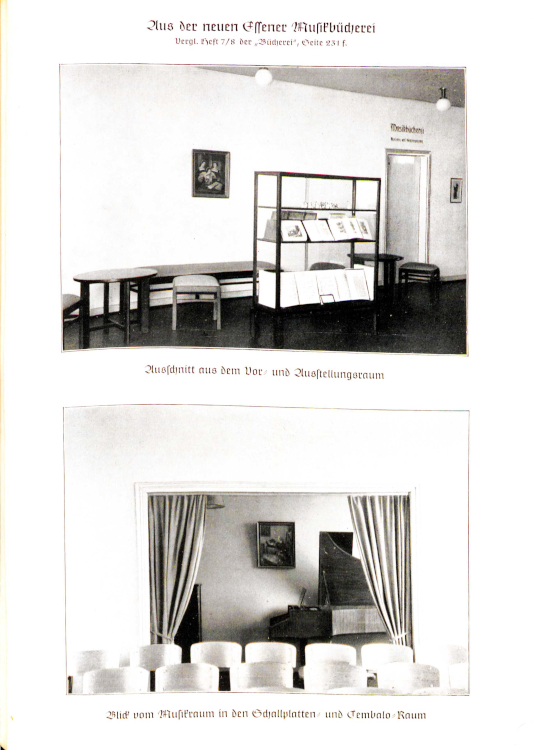
\includegraphics{files/Jansen_1940.jpg}
\caption{Aus der Essener Musikbücherei (Jansen 1940).}
\end{figure}

Dies alles gilt auch für die vier Beiträge, in denen Musikbüchereien
Erwähnung fanden. Bei zwei (Jansen 1940, Schöningh 1941) handelt es sich
um kurz kommentierte Bildbeilagen, welche neu eröffnete Einrichtungen
(Essen, Beuthen) zeigten. Auffällig an diesen ist, dass die Bilder -- im
Gegensatz zu anderen Bildbeilagen, die in der Zeitschrift erschienen --
keine Symbole des Nationalsozialismus zeigen (sonst finden sich zum
Beispiel oft Hakenkreuze oder Bilder von nationalsozialistischen
Führungspersonen). Auch die Beschreibungen gehen vor allem auf den
konkreten Ablauf der Arbeiten in der jeweiligen Bücherei ein. Jansen
(1940), jetzt nicht mehr in Berlin-Charlottenburg, sondern in Essen,
stellt vor allem die Ausleihe der Volksbücherei selber vor («beratende
Thekenausleihe» (Jansen 1940: 279)) und erwähnt die Musikbücherei nur in
einem Nebensatz. Schöningh (1940) geht konkret auf die Arbeit der
Musikbücherei ein (Lesesaal mit Konzertflügel, Fotokopierapparat),
betont dabei aber vor allem, dass die Musikbücherei die «erste
schlesische» (Schöningh 1940: 366) sei. Er fasst dann die Reden, welche
bei der Eröffnungsfeier gehalten wurden, zusammen. Dabei scheint dann
die ideologische Bedeutung, die der Einrichtung zugeschrieben wird,
wieder durch, wenn er die Worte Ministerialrats Dähnhart (vom
\emph{Reichserziehungsministerium}, der dann im Winter 1944 in der
letzten Ausgabe der Zeitschrift auch den einführenden Durchhalteartikel
schreiben wird) wie folgt zusammenfasst:

\begin{quote}
«Das Schwert, das Buch und das Lied sind heute die hauptsächlichen
Träger dieses Ringens {[}um Deutschlands Zukunft{]} und Musik und Buch
Vermittler jener seelischen Kräfte, die den kämpferischen deutschen
Menschen aufs stärkste mit der Heimat verbinden. In diesem Sinne sei
auch die Sonderaufgabe der Beuthener Musikbücherei als Hort
landschaftlicher Musikpflege innerhalb eines Großstadtbüchereiwesens
besonders gegenwartsnah und fruchtbar.» (Schöningh 1940: 367)
\end{quote}

Es entsteht ein wenig der Eindruck, als würden durch die Darstellung der
Arbeit der Büchereien versucht, eine gewisse Normalität zu erzeugen,
während die Realität des nationalsozialistischen Regimes doch immer
wieder durchscheint.

\begin{figure}
\centering
\includegraphics{files/Schöningh_1940_1.jpg}
\caption{Aus der Beuthener Musikbücherei (Schöningh 1940).}
\end{figure}

\begin{figure}
\centering
\includegraphics{files/Schöningh_1940_2.jpg}
\caption{Aus der Beuthener Musikbücherei (Schöningh 1940).}
\end{figure}

Die beiden anderen Beiträge sind Tätigkeitsberichte. Im ersten
(Schermall 1941) wird die Arbeit der Musikbücherei in
Berlin-Charlottenburg, unterstützt mit zahlreichen Zahlen, dargestellt.
Dabei zeigt sich einerseits, dass diese Arbeit nicht nur im Verleih von
Musikalien bestand, sondern auch im Durchführen von «Veranstaltungen,
Konzerten, Hausmusiken und Ausstellungen» (Schermall 1941: 396). Während
die Ausleihe differenziert dargestellt wird -- wohl auch um zu zeigen,
dass anspruchsvolle Musik zur Ausleihe gelangt --, findet die einige
Jahre zuvor explizit vorgestellte «Mittelstelle für Hausmusik» (Jansen
1937) keine Erwähnung mehr. Andererseits enthält der Text jetzt einen
expliziten Verweis darauf, dass diese Musikbücherei nicht während des
Nationalsozialismus gegründet wurde, sondern eine vorhergehende
Tradition hat, über die sonst (Jansen 1937) stillschweigend
hinweggegangen wurde. Schermall schreibt davon, dass die Stadt (Berlin)
die Bibliothek übernommen hätte und dann ein Umbau des Bestandes nötig
gewesen wäre. (Schermall 1941: 396) Er schreibt nicht, wann das
passierte und auch nicht, welche Bibliothek hier übernommen worden war,
aber es ist zu vermuten, dass dies mit der Machtübernahme 1933 zu tun
hatte. Wie weiter oben erwähnt, war Berlin-Charlottenburg in der
Weimarer Republik ein Brennpunkt des Versuchs, die Musikpädagogik zu
demokratisieren. Eventuell stammt der übernommene Bestand aus diesem
Zusammenhang.

Ein letzter Artikel, wieder von Herbert Schermall, erwähnt 1942 einen
«Fortbildungslehrgang für Musikbibliothekare und Musikbibliothekarinnen
in Berlin» (Schermall 1942), der seit 1937/38 an der Berliner
Bibliotheksschule durchgeführt wurde. Der Artikel stellt kurz dar, dass
es notwendig sei, dass die Musikbüchereien von Fachkräften geleitet
werden, welche sowohl eine bibliothekarische Ausbildung als auch Wissen
über Musik hätten. Der Büchereityp sei also so besonders, dass er eine
gesonderte Bildung benötigen würde. Man kann hier von einer gewissen
Professionalisierung des Musikbüchereiwesens reden -- in den
vorhergehenden Jahrzehnten wurde die Frage der notwendigen Kompetenzen
des Personals schon mehrfach angesprochen, jetzt war man zu einer
konkreten Ausbildung übergegangen. Anschliessend wird die Planung und
Durchführung des Lehrgangs dargestellt. Er setzte sich zusammen aus
Vorträgen und Übungen zur bibliothekarischen Arbeit (Bestandsaufbau,
Katalogisierung), aus Vorträgen zur Musikgeschichte und -lehre sowie aus
Musizierstunden. An dem Lehrgang nahmen Musikbibliothekar*innen aus
Berlin sowie «18 Städten Großdeutschlands» (Schermall 1942: 324) teil.
(Das heisst wohl auch aus Städten, die vor 1937 nicht zu Deutschland
zählten, wie vielleicht Wien oder Strassburg.) Diese Zahl -- immerhin
während gleichzeitig Krieg herrschte, also auch viele Personen gar nicht
in ihren «angestammten Berufen» arbeiteten -- deutet ebenso auf eine
nicht geringe Verbreitung der Musikbüchereien hin.

\hypertarget{zur-entwicklung-nach-1945}{%
\section{4. Zur Entwicklung nach
1945}\label{zur-entwicklung-nach-1945}}

Was bis hierher sichtbar wurde, war, dass sich die Frage der Musikalien
in den Volksbüchereien in gewisser Weise mit den Büchereien
mitentwickelt hat. Von ersten Versuchen, zu verorten, welche Position
Musik in den Büchereien haben könnte, über den Aufbau von ersten
Abteilungen bis zum Aufbau von -- wenn man dafür einen später geprägten
Begriff wählt -- musikbibliothekarischen Angeboten, die mit den
zeitgenössischen Aufgaben der Bibliotheken übereinstimmten. Nach 1945
setzte sich dies grundsätzlich fort.

Das Volksbüchereiwesen verortete sich schnell in der «neuen Zeit». Es
baute auf dem auf, was nach 1945 vorhanden war -- nicht nur wurden, wenn
möglich, Büchereigebäude weiter benutzt oder wieder instand gesetzt,
sondern auch Infrastrukturen und Regelungen, die teilweise aus dem
Nationalsozialismus stammten und teilweise aus der Zeit davor, als Basis
akzeptiert, von der aus das neue Volksbüchereiwesen entwickelt wurde.
Was einer Aussonderung unterworfen wurde, waren die Buchbestände. Zum
Teil wurde auch das Personal ersetzt.

Bei diesem Übergang hin zur BRD und DDR wurden auch Debatten und Trends
weiter fortgeführt, aber in einem veränderten Kontext. Schnell bekannten
sich Volksbüchereien zu den neuen Aufgaben -- Demokratie, Humanismus,
Sozialismus --, aber immer auf der Basis der schon etablierten
Arbeitsweisen und Interessen. Mit den Jahrzehnten kam es dann zu einem
massiven Ausbau der Büchereien und zu einer Professionalisierung. Nicht
nur wurden zahllose neue Büchereien und Büchereistandorte geschaffen, in
denen immer mehr professionell ausgebildete Bibliothekar*innen (für die
immer mehr Ausbildungsmöglichkeiten geschaffen wurden) arbeiteten.
Gleichzeitig wurden die Techniken der Büchereien weiterentwickelt und
auch ihre Angebote. Dies weitete sich spätestens in den 1960er- und
1970er-Jahren im gesamten DACH-Raum in den ländlichen Raum aus, so dass
sich eine übergreifende bibliothekarische Versorgung etablierte, die
heute zwar nicht jede Gemeinde, aber doch die meisten erfasst. In dieser
Zeit etablierte sich auch langsam, dass nicht mehr von Volksbüchereien,
sondern Öffentlichen Bibliotheken (in Deutschland), allgemein
öffentlichen Bibliotheken (DDR, Schweiz und Liechtenstein) oder auch
öffentlichen Büchereien (Österreich) gesprochen wurde.

Das Gleiche lässt sich grundsätzlich für die Musikalien und
musikbibliothekarischen Angebote beobachten: Es wurde immer, wie schon
in den Jahrzehnten zuvor, als ein Unterthema des Büchereiwesens
behandelt, das vor allem in grossen Bibliotheken vertreten war, aber dem
vom Bibliothekswesen grundsätzlich immer eine gewisse Sympathie
entgegengebracht wurde. Im Rahmen der allgemeinen Ausweitung der
Öffentlichen Bibliothekswesens und seiner Professionalisierung breitete
sich auch das Musikbibliothekswesen in ihm aus. Dabei wurde den jeweils
aktuellen bibliothekarischen Trends gefolgt.

Ein Beispiel dafür sind zwei Auswahlverzeichnisse von Musikalien, die
beide Ende der 1950er-Jahre in der DDR erschienen. «Mit uns zieht die
neue Zeit Musikbibliothek Dresden» (Stadt- und Bezirksbibliothek Dresden
1958) und «Eine kleine Musikbücherei für dich: Eine Auswahl aus den
Beständen der Musikbibliotheken Halle und Potsdam» (Ruehlmann 1959) sind
beide in gewisser Weise auf der Höhe der Zeit: Sie stellen in Auswahl
dar, welche Musikalien in den genannten Bibliotheken zur Verfügung
stehen. Auswahlverzeichnisse dieser Art waren im Volksbüchereiwesen die
Norm: Es gehörte zur Arbeit der Bibliothekar*innen, solche Verzeichnisse
zu erstellen, ob nun als Typoskript auf Schreibmaschinen oder im Druck,
sowie sie ständig aktuell zu halten. Was sich in den späten 1950ern
allgemein änderte, war, dass man versuchte, in den Verzeichnissen nicht
wenige, ausgewählte, «gute» Medien darzubieten, sondern eine immer
grösser werdende Bandbreite. Den Leser*innen (die in dieser Zeit auch
langsam anders genannt werden) wird immer mehr zugetraut, sich selber in
der Medienlandschaft zu orientieren -- zumindest in einer, die zuvor von
der Bibliothek ausgewählt wurde. Aber nach und nach werden in den
Auswahlverzeichnissen Ende der 1950er nicht mehr einige Dutzend oder
wenige Hundert Medien aufgezählt, sondern möglichst viele -- im
Idealfall alle, die in einer Bibliothek zu einem Thema zur Verfügung
stehen. Damit werden sie umfangreicher, die Anmerkungen, welche die
Medien erläutern, gehen gleichzeitig zurück. Das ist es, was sich auch
in den beiden Auswahlverzeichnissen für Musikalien findet: Das erste ist
noch einige wenige Seiten lang, enthält aber auchschon keine
Besprechungen der aufgeführten Musikalien mehr. Das zweite umfasst fast
100 Seiten von Listen von Musikalien für verschiedene Instrumente sowie
Monografien und Zeitschriften über Musik.

Ein Jahrzehnt später war die Professionalisierung des Öffentlichen
Bibliothekswesen dann weiter fortgeschritten, so auch im
Musikbibliothekswesen -- sichtbar auch daran, dass fast nicht mehr von
«Büchereien», sondern von «Bibliotheken» gesprochen wurde. Es gab
praktisch keine Auswahlverzeichnisse mehr, auch weil die Bestände der
Bibliotheken an sich massiv gewachsen waren. Die Aufgabe der
Bibliothekar*innen war es immer weniger, konkrete einzelne Medien zu
vermitteln, sondern vielmehr ein möglichst breites Medienangebot zur
Verfügung zu stellen und Nutzer*innen dabei zu unterstützen, mit diesen
Medien zu arbeiten. Es gab auch weit mehr Bibliotheken. (Hier sei auf
eine Sammlung der «Musikbibliotheken und Musikaliensammlungen in der
Deutschen Demokratischen Republik» (Thüringer et al., 1969) verwiesen,
die in einer langen Liste nur noch ganze Sammlungen nachweisen kann,
keine einzelnen Medien mehr.)

Diese Ausweitung führte dann auch dazu, dass sich das
Musikbibliothekswesen an sich weiter professionalisierte. Hier sei
wieder auf ein Beispiel verwiesen: die von Alfons Ott 1967 publizierten
«Probleme der musikbibliothekarischen und musikbibliographischen Arbeit:
Zwei Vorträge» (Ott 1967). In diesen geht es nicht mehr um einzelne
Musikbibliotheken oder grundsätzlich die Bedeutung von Musik für
Bibliotheken. Stattdessen fokussierten sie auf Fragen der
Katalogisierung von Musikalien und die Arbeit in Musikabteilungen. Das
ist relevant, weil Ott zu dieser Zeit nicht nur die \emph{Städtische
Musikbibliothek} in München leitete, sondern auch Präsident der
\emph{Commission International des Bibliothèques Musicales Publiques}
war. Schon ein Jahr vorher, 1966, war der \emph{Zeitschriftendienst
Musik} gestartet worden, mit welchem für Musikbibliotheken die
relevanten Zeitschriftenaufsätze gesammelt und verbreitet wurden.

Die Aufgaben in den Musikbibliotheken wurden also immer spezieller, die
eigenständige Ausbildung zur Musikbibliothekar*in, die schon in den
ersten Lehrgängen während des Nationalsozialismus begonnen wurde,
etablierte sich explizit, wenn auch immer prekär -- so gibt es heute
wieder weniger spezifische Ausbildungsgänge und Fortbildungen, als noch
im Artikel von Diet (2013) erwähnt wurden. 1980 wurde dann vom
\emph{Deutschen Bibliotheksinstitut} mit dem \emph{Forum
Musikbibliothek} eine eigene Zeitschrift für diesen Bibliothekstyp --
allerdings nicht nur für die Öffentlichen, sondern für alle Formen von
Musikbibliotheken -- in der BRD gegründet. Im Gegensatz zu vielen
anderen Zeitschriften, welche das Institut während seines Bestehens
gründete, überlebte das \emph{Forum Musikbibliothek} dessen Schliessung
im Jahr 2000 und erscheint bis heute. Allerdings scheint mit dieser
Gründung auch die Zeit vorbei gewesen zu sein, in welcher zumindest in
den allgemeinen bibliothekarischen Zeitschriften der BRD und dann nach
1989 Deutschlands, Musikalien und Musikbibliotheken regelmässig zum
Thema von Artikeln wurden. Es scheint, es wäre der Bibliothekstyp so
eigenständig geworden, dass er von anderen Bibliothekstypen nicht (mehr)
integriert, sondern als eigenständig wahrgenommen wird.

Blickt man aber die Ausgaben der Zeitschrift aus den letzten Jahren
durch, dann scheint sich auch weiterhin zu zeigen, dass sich das
öffentliche Musikbibliothekswesen mit den Trends des Öffentlichen
Bibliothekswesens mitentwickelt. Neben Darstellungen von
Digitalisierungsprojekten Wissenschaftlicher Bibliotheken und
historischen Arbeiten finden sich dort heute zum Beispiel Berichte über
öffentliche Musikveranstaltungen mit (Blase 2022) und ohne
Erziehungsanspruch (Straka 2023), über Empfehlungslisten (Wilke 2022)
und Makerspaces in öffentlichen Musikbibliotheken. (Gründler 2023)

\hypertarget{fazit-gemeinsame-entwicklungslinien}{%
\section{5. Fazit: Gemeinsame
Entwicklungslinien}\label{fazit-gemeinsame-entwicklungslinien}}

Schaut man auf die Entwicklungen zurück, die in diesem Artikel
geschildert wurden, dann zeigen sich einige klare Entwicklungslinien des
Musikbüchereiwesens -- oder, wie man heute eher sagen würde, des
öffentlichen Musikbibliothekswesens. Zuerst ist sichtbar, dass Musik in
gewisser Weise immer ein Thema des Büchereiwesens war. Von Beginn an
galt es als ein Thema, welchem in der betreffenden Fachpresse und der
Praxis der Büchereien Platz eingeräumt wurde. Auch wenn sich immer
wieder Hinweise darauf finden, dass es dazu Gegenstimmen gegeben hätte,
welche die «Musikalien» nicht als Teil des Büchereibestandes ansahen,
lassen sich diese Gegenstimmen nirgends wirklich nachweisen. Sie
erscheinen immer als Erzählung Dritter; so, als wären sie eher ein
Mythos. Was sich vielmehr findet, ist eine Affinität des Büchereiwesens
zur Musik. Allerdings immer mit der Einschränkung, dass Musik nicht als
das wichtigste Thema der Diskussionen und Praxis galt. Im Vergleich zur
gesamten Literatur waren es immer nur einige Artikel und im Vergleich
zur Zahl der Büchereien waren es immer nur einige Büchereien, die auch
Musikabteilungen oder eigenständige Musikbüchereien einrichteten.
Sicherlich: In den Jahrzehnten nach 1945 änderte sich auch dies und die
Musikabteilung wurde zum normalen Teil einer Öffentlichen Bibliothek,
inklusive einer eigenständigen Ausbildung für Musikbibliothekar*innen,
die sich in den hier besprochenen Texten auch schon andeutete. Aber halt
doch immer als eine Einrichtung, die neben dem «Hauptgeschäft» betrieben
wurde -- als Teil des Büchereiwesens akzeptiert und doch immer
spezialisiert.

Gleichzeitig zeigte sich, dass die Entwicklung der Musikbüchereien die
des gesamten Büchereiwesens spiegelt. So, wie das Büchereiwesen sich
zuerst als Erziehungswesen begriff und von «reiner Unterhaltung»
abgrenzte, galt dies auch für Musikbüchereien. So, wie im Büchereiwesen
kontinuierlich versucht wurde, mit jeweils moderner Technik und einer
sich ausweitenden Veranstaltungsarbeit die selbstgestellten Aufgaben
immer besser zu erfüllen, galt dies auch für die Musikbüchereien. Und
leider so, wie das Volksbüchereiwesen sich relativ einfach in das
nationalsozialistische System integrieren liess, galt dies ebenso für
die Musikbüchereien. Auch das wird sich dann in den Jahrzehnten nach
1945 fortsetzen. So, wie die Büchereien erst langsam, dann spätestens ab
Ende der 1960er-Jahre immer schneller offener wurden, wurden es auch die
Musikbüchereien. Und so, wie Büchereien sich mit der Zeit immer mehr
auch als Einrichtungen zur Freizeitgestaltung verstanden, galt dies wohl
ebenso für die Musikabteilungen. Es ist zu erwarten, dass sich eine
solche Parallelität auch in Zukunft zeigen wird: Die Musikbibliotheken
werden sich mit den Öffentlichen Bibliotheken mitentwickeln, aber als
eine Sonderform.

Ein Trend, der auch das Schreiben dieses Textes hier schwierig machte,
ist, dass sich über die ganze Zeit keine eindeutige Bezeichnung für die
Musikbüchereien durchsetzte. Sie wurden je nach lokaler Gegebenheit und
wohl auch der Vorlieben der Autor*innen, unterschiedlich benannt.
Teilweise zeigt sich dabei die Schwierigkeit, dass sie unterschiedlich
organisiert waren: Mal als Abteilungen, mal als eigenständige Büchereien
und manchmal als Einrichtungen «zwischen» diesen beiden Lösungen. Der
Begriff «Musikbücherei» wurde hier in diesem Artikel bei der
historischen Darstellung als Hauptbegriff gewählt, weil sich so weitere
Unübersichtlichkeiten vermeiden liessen. Aber auch das scheint bis heute
für die Musikbibliotheken zu gelten: Es ist nicht eindeutig klar,
«wohin» sie gehören. Sind sie eine Abteilung, die Personal mit oder ohne
spezifischen Kenntnissen bedarf? Sind sie ein eigener Bibliothekstyp?
Sind sie -- das ist der Ansatz, dem zum Beispiel bei der heutigen
Zeitschrift \emph{Forum Musikbibliothek} gefolgt wird -- ein
Bibliothekstyp, der quer liegt zur Typologie Öffentliche
Bibliothek/Wissenschaftliche Bibliothek/Spezialbibliothek oder gibt es
eher verschiedene Formen von Musikbibliotheken, also Öffentliche,
Wissenschaftliche und eigenständige Musikbibliotheken mit jeweils
unterschiedlichen Aufgaben? Wenn es einen erkennbaren Trend gibt, der
sich zu Beginn des 20. Jahrhunderts abzeichnete und auch noch heute
finden lässt, dann den, dass diese Frage nie vollständig geklärt wird.

***

Um am Ende auf die Frage zurückzukommen, die Wilhelm Altmann 1900
stellte -- die, ob Musikalien in die Bücherhallen gehören -- kann man
jetzt, mehr als 120 Jahre später sagen: Ja, das tun sie offenbar. Das
Hauptmedium von «Bücherhallen» ist weiterhin, wie zu Altmanns Zeiten,
das gedruckte Buch. Andere Medienformen sind dazugekommen, einige --
denken wir nur an die Videokassetten -- sind praktisch schon wieder
verschwunden. Aber die «Musikalien», die bleiben offenbar -- wenn auch
vielleicht in anderen Medientypen als den Notendrucken, die Altmann
bevorzugte. Die Öffentliche Bibliothek heute ist also, wie Altmann
forderte, auch eine Musikbibliothek, offenbar weil es -- bei allen
Veränderungen über die Jahrzehnte -- daran weiterhin ein Interesse von
Nutzer*innen und Bibliothekar*innen gibt.

\hypertarget{literatur}{%
\section{Literatur}\label{literatur}}

Ackerknecht, Erwin 1930. Bildungspflege und Schallplatte. \emph{Bücherei
und Bildungspflege: Zeitschrift für die gesamten außerschulischen
Bildungsmittel} 10, 1, 7--15.

Ackerknecht, Erwin 1924. \emph{Büchereifragen}. Berlin: Weidmannsche
Buchhandlung.

Ackerknecht, Erwin 1926. \emph{Vorlesestunden}. 2. Auflage. Berlin:
Weidmannsche Buchhandlung.

Altmann, Wilhelm 1900. Gehören Musikalien in die Bücherhallen?
\emph{Blätter für Volksbibliotheken und Lesehallen} 1, 3--4, 41--45.

Angermann, Rudolf 1937a. Die Musikbücherei. \emph{Die Bücherei:
Zeitschrift für Schriftumspflege} 4, 7--8, 301--310.

Angermann, Rudolf 1937b. Die Musikbücherei. \emph{Die Bücherei:
Zeitschrift für Schriftumspflege} 4, 9--10, 387--397.

Barbian, Jan-Pieter 2010. \emph{Literaturpolitik im NS-Staat: Von der
Gleichschaltung bis zum Ruin}. Frankfurt am Main: Fischer Taschenbuch
Verlag.

Bayer, Karl Th. 1931. Musik und Bücherei. \emph{Bücherei und
Bildungspflege: Zeitschrift für die gesamten außerschulischen
Bildungsmittel} 11, 3, 176--184.

Blase, Axel 2022. Menschen mit Musik verbinden. Über den Beginn des
Projektes „Gemeinsam InTakt - mit Veeh-Harfen die Welt der Musik
entdecken'' in der Stadtbibliothek Reutlingen. \emph{Forum
Musikbibliothek} 43, 1, 7--12.

Dähnhardt, Heinz 1938a. Richtlinien für das Volksbüchereiwesen.
\emph{Die Bücherei: Zeitschrift für Schriftumspflege} 5, 1, 1--7.

Dähnhardt, Heinz 1938b. Richtlinien für das Volksbüchereiwesen.
\emph{Die Bücherei: Zeitschrift für Schriftumspflege} 5, 3, 130--136.

Dähnhardt, Heinz 1944. Warum bleiben die Büchereien geöffnet? \emph{Die
Bücherei: Zeitschrift für Schriftumspflege} 11, 10--12, 297--301.

Der Herausgeber 1900. Zur Einführung. \emph{Blätter für
Volksbibliotheken und Lesehallen} 1, 1, 1--4.

Der Reichs- und Preußische Minister für Wissenschaft, Erziehung und
Volksbildung 1938. Richtlinien für das Volksbüchereiwesen. \emph{Die
Bücherei: Zeitschrift für Schriftumspflege} 5, 1, 39--46.

Diet, Jürgen 2013. Musikbibliothekarische Aus- und Fortbildung in
Deutschland. \emph{Forum Musikbibliothek} 34, 3, 24--28.

Eschen, Andreas 2008. Kestenberg und die Jugendmusikbewegung: Von der
Reichsschulkonferenz und Jödes Musikalische Jugendkultur bis zur
Ernneung Jödes zum Professor. In S. Fontaine u.~a., hg. \emph{Leo
Kestenberg: Musikpädagoge und Musikpolitiker in Berlin, Prag und Tel
Aviv}. Rombach Wissenschaften. Reihe Litterae. Freiburg im Breisgau;
Berlin; Wien: Rombach Verlag, 69--87.

Fackler, Guido 2000. „\emph{Des Lagers Stimme'' - Musik im KZ: Alltag
und Häftlingskultur in den Konzentrationslagern 1933 bis 1936\,: mit
einer Darstellung der weiteren Entwicklung bis 1945 und einer
Biblio-/Mediographie}. Bremen: Edition Temmen.

Gesamtvorstand der Comenius-Gesellschaft 1899. Schafft Bücherhallen!
\emph{Comenius-Blätter für Volkserziehung} 7, 5--6, 67--74.

Gilbert, Shirli 2005. \emph{Music in the Holocaust: confronting life in
the Nazi ghettos and camps}. Oxford: Clarendon Press.

Gründler, Felix 2023. Konzeption und Einrichtung eines Makerspace in
einer öffentlichen Musikbibliothek am Beispiel von NEXT LEVEL in der
Stadtbücherei Augsburg. \emph{Forum Musikbibliothek} 44, 1, 30--35.

Hanauer, J 1907. Erfahrungen und Vorschläge für Musikalien-Bibliotheken.
\emph{Blätter für Volksbibliotheken und Lesehallen} 8, 5--6, 76--79.

Hanauer, J. 1905. Von der Musikalien-Frei-Bibliothek in Frankfurt a.M.
\emph{Blätter für Volksbibliotheken und Lesehallen} 6, 9--10, 145--149.

Hecker, Konrad 1943. Die Aufgabe des Katalogs. \emph{Die Bücherei:
Zeitschrift für Schriftumspflege} 10, 1--3, 3--19.

Heiligenstaedt, Fritz 1938a. Die Schülerbücherei im Rahmen
nationalsozialistischer Erziehungsarbeit. \emph{Die Bücherei:
Zeitschrift für Schriftumspflege} 5, 7--8, 404--409.

Heiligenstaedt, Fritz 1938b. Volksbibliothekarische Zusammenarbeit.
Vortrag, gehalten auf dem Deutschen Volksbüchereitag Leipzig 1938.
\emph{Die Bücherei: Zeitschrift für Schriftumspflege} 5, 11, 656--670.

Hofmann, Hans \& Ameln, Konrad 1927. Musik in der volkstümlichen
Bücherei. \emph{Hefte für Büchereiwesen} 11, 2, 71--79.

Holz, Mia 2019. \emph{Musikschulen und Jugendmusikbewegung: Die
Institutionalisierung des öffentlichen Musikschulwesens von den 1920ern
bis in die 1960er-Jahre}. Münster: Waxmann Verlag.

Jansen, Carl 1937. Die Musikbücherei als Mittelstelle für
Hausmusikpartner. \emph{Die Bücherei: Zeitschrift für Schriftumspflege}
4, 9--10, 398--401.

Jansen, {[}Carl{]} 1940. Essens neue Volksbücherei-Hauptstelle: zu
unserer Bildbeilage. \emph{Die Bücherei: Zeitschrift für
Schriftumspflege} 7, 9, 279.

Klapp, Wilhelm 1938. Vom deutschen Musikbüchereiwesen. \emph{Die
Bücherei: Zeitschrift für Schriftumspflege} 5, 2, 65--72.

Klause, Inna 2021. „\emph{Und alles mit Musikbegleitung'': Musikausübung
im Gulag und in den nationalsozialistischen KZ im Vergleich}. Wiesbaden:
Harrassowitz Verlag.

Löwe, Hans 1938. Die Aufgaben einer Gefängnisbücherei. \emph{Die
Bücherei: Zeitschrift für Schriftumspflege} 5, 5, 276--283.

Mahlert, Ulrich 2008. Leo Kestenberg und das Seminar für Musikerziehung
an der Berliner Hochschule für Musik: Einblicke und Ausblicke. In S.
Fontaine u.~a., hg. \emph{Leo Kestenberg: Musikpädagoge und
Musikpolitiker in Berlin, Prag und Tel Aviv}. Rombach Wissenschaften.
Reihe Litterae. Freiburg im Breisgau; Berlin; Wien: Rombach Verlag,
89--117.

Marsop, Paul 1916. Von den Volksbüchereien für Musik. \emph{Blätter für
Volksbibliotheken und Lesehallen} 17, 1--2, 1--2.

Meier, Franziska 2022. \emph{Ein „bündischer Kulturmarkt'' entsteht: Die
deutsche Jugendbewegung und Jugendmusikbewegung als Katalysator für den
Aufbau von Kulturmarktunternehmen 1918-1933}. Stuttgart: Franz Steiner
Verlag.

Michalzik, Peter 2018. \emph{1900: Vegetarier, Künstler und Visionäre
suchen nach dem neuen Paradies}. Erste Auflage. Köln: DuMont.

Nierenz, Heike 2010. \emph{Musik in den Ritualen einer Ersatzreligion:
Der Nationalsozialismus und seine Gemeinschaftslieder - musikalische
Analysen}. Marburg: Tectum Verlag.

Niessen, Anne 1999. „\emph{Die Lieder waren die eigentlichen
Verführer!{}``: Mädchen und Musik im Nationalsozialismus}. Mainz\,;
London\,; Madrid\,; New York\,; Paris\,; Tokyo\,; Toronto: Schott Musik
International.

Ott, Alfons 1967. \emph{Probleme der musikbibliothekarischen und
musikbibliographischen Arbeit: Zwei Vorträge}. Berlin: Deutscher
Büchereiverband, Arbeitsstelle für das Büchereiwesen.

Otten, Bennata 1913. \emph{Bibliothekstechnischer Ratgeber für
Volksbibliotheken, Lesehallen und verwandte Büchereie\,: mit
Bibliographie der Fachliteratur von 1900 - 1912}. Leipzig: Harrassowitz
Verlag.

Petit, Élise 2018. \emph{Musique et politique en Allemagne, du IIIe
Reich à l'aube de la guerre froide}. Paris: Presses de l'universitö
Paris-Sorbonne.

Pfoser, Alfred 1980. \emph{Literatur und Austromarxismus}. Wien: Löcker
Verlag.

Pöggeler, Franz (Hg.) 1974. \emph{Geschichte der Erwachsenenbildung}.
Stuttgart: Kohlhammer.

Rathkolb, Oliver 2020. Zeithistorische Anmerkungen zur Geschichte der
Musikschule der Stadt Wien 1938-1945. Eine nationalsozialistische
Gründung auf den Trümmern von drei privaten Konservatorien. In S. Zapke
u.~a., hg. \emph{Die Musikschule der Stadt Wien: Eine "ideologische
Lehr- und Lerngemeinschaft}. Wien: Hollitzer Verlag, 15--53.

Reichsstelle für das Volksbüchereiwesen 1938. \emph{Reichsliste für
Musikbüchereien}. Leipzig: Einkaufshaus für Büchereien.

Richter, Christoph 2008. Leo Kestenbergs Reformutopien als Anregung und
Aufgabe für die Gestaltung unseres Musiklebens. In S. Fontaine u.~a.,
hg. \emph{Leo Kestenberg: Musikpädagoge und Musikpolitiker in Berlin,
Prag und Tel Aviv}. Rombach Wissenschaften. Reihe Litterae. Freiburg im
Breisgau; Berlin; Wien: Rombach Verlag, 159--175.

Rindlisbacher, Stefan 2022. \emph{Lebensreform in der Schweiz
(1850--1950): Vegetarisch essen, nackt baden und im Grünen wohnen}.
Bern: Peter Lang.

Rothhardt, Hans 1926. \emph{Das erste Jahrfünft der Stadtbücherei
Berlin-Steglitz: Bericht anläßlich ihres fünfjährigen Bestehens am 1.
Oktober 1925}. Berlin: W. Zieger.

Rothhardt, Hans 1911. Die Verleihung von Musikalien durch
Volksbüchereien. \emph{Blätter für Volksbibliotheken und Lesehallen} 12,
9--10, 133--136.

Rothhardt, Hans 1909. \emph{Meine lieben vier Wände: Gedichte}. Leipzig:
Karl Lentze Verlag.

Rothhardt, Hans 1923. \emph{Musikgärtlein}. Berlin: Orplid-Verlag.

Ruehlmann, L. (Hg.) 1959. \emph{Eine kleine Musikbücherei für dich: Eine
Auswahl aus den Beständen der Musikbibliotheken Halle und Potsdam}.
Halle (Saale): Kreuz-Verlag.

Schermall, Herbert 1941. Aus der Musikbücherei Berlin-Charlottenburg.
\emph{Die Bücherei: Zeitschrift für Schriftumspflege} 8, 11, 396--399.

Schermall, Herbert 1942. Fortbildungslehrgang für Musikbibliothekare und
Musikbibliothekarinnen in Berlin. \emph{Die Bücherei: Zeitschrift für
Schriftumspflege} 9, 9--12, 322--325.

Schöningh 1941. Zur Eröffnung der Beuthener Musikbücherei (Siehe
Bildbeilage). \emph{Die Bücherei: Zeitschrift für Schriftumspflege} 8,
10, 366--367.

Schriewer, Franz 1938. Leistungszahlen der Schülerbüchereien. \emph{Die
Bücherei: Zeitschrift für Schriftumspflege} 5, 6, 340--342.

Schuster, Wilhelm 1934. Die Neuordnung des Preußischen Büchereiwesens.
\emph{Die Bücherei: Zeitschrift für Schriftumspflege} 1, 1, 9--17.

Seidl, Johann Wilhelm 1989. \emph{Musik und Austromarxismus: Zur
Musikrezeption der österreichischen Arbeiterbewegung im späten
Kaiserreich und in der Ersten Republik}. Wien: Böhlau Verlag.

Stadt- und Bezirksbibliothek Dresden (Hg.) 1958. \emph{Mit uns zieht die
neue Zeit Musikbibliothek Dresden}. Dresden: Stadt- u. Bezirksbibliothek
Dresden.

Stoverock, Karin 2013. \emph{Musik in der Hitlerjugend: Organisation,
Entwicklung, Kontexte}. Bd. 1/2, Uelvesbüll: Der andere Verlag.

Straka, Beate 2023. Balkonkonzerte und MusikGespräche in der
Stadtbibliothek Stuttgart. \emph{Forum Musikbibliothek} 44, 2, 12--16.

Thier, Erich 1943. Im Dickicht der Kataloge. \emph{Die Bücherei:
Zeitschrift für Schriftumspflege} 10, 4--6, 98--117.

Thüringer, Peter (Hg.) 1969. \emph{Musikbibliotheken und
Musikaliensammlungen in der Deutschen Demokratischen Republik}. Berlin:
Deutscher Bibliotheksverband, Sektion Musikbibliotheken.

Trippen, Norbert 1996. 150 Jahre katholische Büchereiarbeit. Von der
Gründung des Borromäusvereins 1845 bis zu seiner Neustrukturierung 1995.
In N. Trippen \& H. Patenge, hg. \emph{Bausteine für eine lesende
Kirche: Borromäusverein und katholische Büchereiarbeit\,; Festgabe für
Erich Hodick}. Mainz: Matthias Grünewald Verlag, 36--52.

Weiß-Reyscher, Elisabeth 1938. \emph{Anweisung zur Titelaufnahme von
Musikalien}. Leipzig: Einkaufshaus für Büchereien.

Wilke, Sebastian 2022. Musikempfehlungen und kuratierte Inhalte über
Spotiy - Erste Erfahrungen aus der Stadtbücherei Frankfurt am Main.
\emph{Forum Musikbibliothek} 43, 2, 16--20.

Zalar, Jeffrey T. 2019. \emph{Reading and rebellion in Catholic Germany,
1770-1914}. Cambridge: Cambridge University Press.

Zapke, Susana 2020. Musik zur Volkserhebung und seelischen Kräftigung:
Zur Programmatik der Musikschule der Stadt Wien. In S. Zapke u.~a., hg.
\emph{Die Musikschule der Stadt Wien: Eine "ideologische Lehr- und
Lerngemeinschaft}. Wien: Hollitzer Verlag, 55--81.

Zoumer, Jakob 1931. Der Volksbildungsabend und die Musik. In J.
Zimmermann, hg. \emph{Vorlesestunden und Volksbildungabende: Anleitung,
Dichtung und Vortragsfolgen}. Bonn: Verlag des Borromäusvereins, 57--62.

%autor
\begin{center}\rule{0.5\linewidth}{0.5pt}\end{center}

\textbf{Dr.~Karsten Schuldt}, wissenschaftlicher Projektleiter am
Schweizerischen Institut für Informationswissenschaft, Fachhochschule
Graubünden (Chur) und Redakteur der LIBREAS. Library Ideas.

\end{document}